\chapter{Sistemi Complessi}
\section{Introduzione}
Verranno trattati degli stumenti per modellare e descrivere fenomeni naturali e reali
che variano nel tempo
\begin{definizione}[\textbf{Sistema complesso}]
    Un \textbf{Sistema complesso} è un insieme di unità semplici che cooperano tra
    di loro facendo emergere dei comportamenti complessi.
\end{definizione}
Verranno analizzati modelli discreti che sono facilmente implementabili utilizzati
nelle simulazioni, un sesempio sono:
\begin{itemize}
    \item \textbf{Automi cellulari}: paridigma di calcolo locale, parallelo e omogeneo
    \item \textbf{Subshift}: modelli per definire sistemi di condifica basata su
          parole proibite
    \item \textbf{Tiling}: modelli basati sul problema del tiling, ovvero ricoprire
          una superficie con delle piastrelle in modo tale che combaciano i colori sui
          lati di due piastrelle omogenee (problema NP-Hard).
\end{itemize}

Si studieranno le proprietà dei fenomeni reali utilizzando i modelli e si mapperanno
le domande sulle proprietà dei modelli, in questo modo si potrà rispondere alle
domande analizzando le proprietà dei modelli.

\section{Automi cellulari (alfabeto finito)}
Gli automi cellulari sono delle reti di automi, gli automi, non per forza a stati
finiti, di cui sono composte possono essere uguali (automi cellulari uniformi) o differenti (automi cellulari non
uniformi). Lo stato dell'automa cellurare in un particolare momento dell'esecuzione
sarà l'insieme degli stati dei singoli automi nel particolare momento.

\begin{nota}
    Si parla di insieme degli stati del singolo automa perché può essere una
    sequenza nel caso di CA 1D, una matrice nel caso CA 2D, ecc$\dots$
\end{nota}

La transizione dell'automa cellulare dipende direttamente dalle transizioni dei singoli automi,
i quali, quando scattano, leggono il loro stato interno e gli stati degli automi
vicini e cambiano stato di conseguenza. Il cambio della configurazione dell'automa
cellulare coincide col cambiamento di stato di tutti gli automi della rete contemporaneamente.
Per questo gli automi cellulari sono un paradigma di calcolo:
\begin{itemize}
    \item locale
    \item parallelo
    \item uniforme (non uniforme)
\end{itemize}

\begin{nota}
    Gli automi cellulari sono dei paradigmi di calcolo universale perché si
    può convertire una qualsiasi Macchina di Turing in un automa cellulare
\end{nota}

\begin{nota}
    Gli automi cellulari sono delle reti di automi, un esempio di rete di automi
    è la rete neurale, in questo caso:
    \begin{itemize}
        \item non è uniforme perché ogni neurone può avere una funzione differente
        \item non è locale perché ogni neurone può non dipendere solo dai neuroni
              vicini
        \item è parallelo perché i neuroni scattano contemporaneamente
    \end{itemize}
\end{nota}

\begin{definizione} [\textbf{sequenze bi-infinite}]
    Dato un alfabeto $A$, chiameremo \textbf{sequenze bi-infinite} sull'alfabeto
    $A$ tutte quelle sequenze che sono infinite a destra ed infinite a sinistra.
\end{definizione}

\begin{esempio}
    Sia $A = \left\{0,1\right\}$ allora:
    \begin{itemize}
        \item $01101001110011$: è una sequenza finita
        \item $01101001110011\dots$: è una sequenza infinita a destra
        \item $\dots01101001110011$: è una sequenza infinita a sinistra
        \item $\dots01101001110011\dots$: è una sequenza bi-infinita
    \end{itemize}
\end{esempio}

\begin{definizione}[\textbf{spazio delle configurazioni}]
    Lo \textbf{spazio delle configurazioni} è
    $$A^\mathbb{Z}= \left\{x|x:\mathbb{Z}\rightarrow A\right\}$$
    Coincide con l'insieme di tutte le sequenze \textbf{bi-infinite} sull'alfabeto
    $A$
\end{definizione}
Lo spazio delle configurazioni è un insieme di funzioni, ciascuna funzione rappresenta
una sequenza \textbf{bi-infinita} che associa ad ogni indice in $\mathbb{Z}$ della
sequenza un carattere dell'alfabeto.
\begin{esempio}
    Sia $x\in A^\mathbb{Z}$, si può rappresentare nel sequente modo
    $$x = \left(\dots, x_{-2}, x_{-1},x_{0},x_{1},x_{2},\dots\right), \ \forall x_i\in A$$
    Con
    $$x(i) = x_i$$
\end{esempio}

Si studiano automi cellulari infiniti perché possono catturare tutti i comportamenti
del sistema, cosa che non posso fare con gli automi finiti. Essendo infiniti,
le singole configurazioni dell'automa devono essere infite, ecco perché si utilizzano
\textbf{sequenze bi-infinite}.

\begin{definizione} [\textbf{sottosequenza}]
    Possiamo definire le \textbf{sottosequenza} di una \textbf{sequenza bi-infinita}
    nel seguente modo.

    $\forall x \in A^{\mathbb{Z}}$ e $\forall h,k\in \mathbb{Z}$ con $h\le k$
    abbiramo:
    $$x_{[h,k]}= x_hx_{h+1}\dots x_k\in A^{k-h+1}$$
    La sottosequenza sarà finita e di lunghezza $k-h+1$.
\end{definizione}

Per studiare alcune proprietà degli automi cellulari si utilizzano i concetti di
distanza.
\begin{definizione}[\textbf{distanza su un generico insieme}]
    Dato un insieme $X$, una \textbf{funzione distanza} è una qualsiasi funzione
    $d:X\times X \rightarrow \mathbb{R}_+$ che soddisfa le sequenti proprietà:
    \begin{itemize}
        \item \textbf{non degenerazione}: $\forall x,y\in X, d(x,y) = 0\iff x=y$
        \item \textbf{simmetrica}: $\forall x,y\in X, d(x,y) = d(y,x)$
        \item \textbf{disuguaglianza triangolare}: $\forall x,y,z\in X, d(x,y) \le d(x,z)+d(z,y)$
    \end{itemize}
\end{definizione}

\begin{esempio}[distanza triviale]
    Un esempio di distanza è la seguente
    $$d(x,y) =\begin{cases}
            0 & x=y    \\
            1 & x\ne y \\
        \end{cases}$$
\end{esempio}

\begin{esempio}[distanza euclidea]
    Un esempio di distanza è la seguente
    $$d(x,y) =|x-y|$$
    Generalizzabile su $\mathbb{R}^n$ con la $|.|_2$$\dots$
\end{esempio}

A noi servirà una distanza tra le configurazioni di CA per poter confrontare
la vicinanza tra di loro e studiare le varie proprietà, utilizzeremo la distanza di
\textbf{Tychonoff}.
\begin{definizione} [\textbf{distanza su $A^\mathbb{Z}$}]
    $d:A^\mathbb{Z}\times A^\mathbb{Z} \rightarrow \mathbb{R}_+$ definita nel
    seguente modo:
    $$d(x,y) = \begin{cases}
            0             & x=y        \\
            \frac{1}{2^n} & altrimenti
        \end{cases}$$
    Dove $n= \min\left\{k\in \mathbb{N} | x_{[-k,k]} \ne y_{[-k,k]}\right\}$
\end{definizione}

La distanza si può anche non centrare nello $0$ ma in un altro indice differente,
ovviamente il calcolo cambia. Sia $d_i$ la distanza con il calcolo di $n$ centrato
in $i$ allora per ottenere $n$ si prende il valore $n'$ centrato in $i$ e si somma
l'offset dall'indice $0$.

\begin{nota} [Proprietà $1$ della distanza] \label{prop:dist}
    $\forall x,y\in A^\mathbb{Z}$, $\forall n\in \mathbb{N}$ vale che
    $$d(x,y)< \frac{1}{2^n}\iff x_{[-n, n]}=y_{[-n, n]}$$
\end{nota}

\begin{definizione}
    $(A^\mathbb{Z}, d)$ è lo \textbf{spazio metrico} delle configurazioni dell'automa
\end{definizione}

\begin{nota} [Proprietà $2$ della distanza]
    $(A^\mathbb{Z}, d)$ è un \textbf{spazio metrico compatto} cioè ogni successione
    di elementi di $A^\mathbb{Z}$ ammette una sottosuccessione convergente in $A^\mathbb{Z}$.
\end{nota}


\begin{definizione} [ \textbf{Automa cellulare 1D} ]
    Un \textbf{Automa cellulare 1D}  è una tripla $\langle A, r, f\rangle$
    dove:
    \begin{itemize}
        \item $A$: insieme finito di caratteri, corrisponde all'alfabeto dell'automa e
              quindi agli stati degli automi interni.
        \item $r\in \mathbb{N}$: raggio degli automi interni, specifica il raggio
              di dipendenza degli automi interni da quelli vicini. La transizione degli
              automi interni sarà dipendente dagli stati degli automi nel raggio
              di vicinanza $r$.
        \item $f: A^{2r+1}\rightarrow A$: regola locale di aggiornamento dello
              stato degli automi interni.
    \end{itemize}
\end{definizione}
Ad ogni $CA = \langle A, r, f\rangle$ viene associata una $F:A^\mathbb{Z}\rightarrow A^\mathbb{Z}$
chiamata \textbf{regola globale} che coincide con la specifica del cambiamento
di configurazione del $CA$.
\begin{definizione} [\textbf{Regola globale per CA}]
    $F:A^\mathbb{Z}\rightarrow A^\mathbb{Z}$, dati $\forall x \in A^\mathbb{Z}, i \in \mathbb{Z}$
    si definisce
    $$F(x)_i = f(x_{[i-r, i+r]})$$
    quindi
    \begin{table}[!h]
        \centering
        \begin{tabular}{ccccccccccc}
            $x$    & $=$ & $($ & $\dots$                     & $x_{i-r}$ & $\dots$                     & $x_i$ & $\dots$ & $x_{i+r}$ & $\dots$ & $)$ \\
            $F(x)$ & $=$ & $($ & \multicolumn{3}{c}{$\dots$} & $F(x)_i$  & \multicolumn{3}{c}{$\dots$} & $)$
        \end{tabular}
    \end{table}
\end{definizione}
\begin{definizione} [ \textbf{Automa cellulare 1D elementare} ]
    Gli \textbf{Automi cellulari 1D elementari} sono \textbf{Automi cellulari 1D}
    con $A=\{0,1\}$ e $r=1$
\end{definizione}

Più precisamente per rappresentare un CA  $\langle A, r, f\rangle$ ci sono 3 modi:
\begin{itemize}
    \item \textbf{tabella}: si scrive la tabella che definisce la regola locale
    \item \textbf{numero decimale}: si utilizza un numero decimale che condifica
          la regola locale, si può ricavare facilmente dalla tabella
          $$n_f = \{0,\dots, |A|^{|A|^{2r+1}-1}\}$$
    \item \textbf{grafo di De Bruijn}: si utilizza un grafo orientato
\end{itemize}


\begin{esempio} [Rappresentazione tabellare]
    Per rappresentare la regola locale in tabella, basta creare una tabella di
    $|A|^{2r+1}$ righe e $2$ colonne. Nella prima colonna si mettono per riga e in ordine
    tutte le combinazioni di input, nella seconda colonna si mette il carattere
    finale.
\end{esempio}

\begin{esempio} [Rappresentazione numero decimale]
    Per rappresentare la regola locale in numero decimale, basta rappresentare
    la regola locale in tabella e poi codificare in decimale il numero scritto in
    verticale dal basso verso l'alto nella seconda colonna. Ricorda che questo numero
    è in base $|A|$.
\end{esempio}

\begin{nota}
    Per gli CA elementari si ha che la regola locale è defina nel seguente modo
    $$f:\{0,1\}^3\rightarrow \{0,1\}$$
    Quindi si possono avere un totale di $256 = |\{0,1\}^3|
        = |C|^{|D|}$ regole locali che
    corrispondono quindi a $256$ CA 1D elementari e ogni automa è rappresentato da un
    numero $x\in [0, 255]$ che corrisponde alla conversione in decimale della regola
    locale.
\end{nota}

\begin{definizione} [\textbf{Grafo di De Bruijn}]
    Il \textbf{Grafo di De Bruijn} associato a CA $\langle A, r, f\rangle$ è $\langle V,E,l\rangle$
    dove:
    \begin{itemize}
        \item $V=A^{2r}$
        \item $E = \{(u,v)\in V\times V | u=u_1\dots u_{2r},  v=v_1\dots v_{2r} \text{ con } u_2\dots u_{2r} = v_1\dots v_{2r-1}\}$
        \item $l:E\rightarrow \{0,1\}$ funzione che etichetta gli archi nel seguente
              modo $$\forall (u,v)\in E, l(u,v) = f(u,v_{2r})=f(u_1,v)$$
    \end{itemize}
\end{definizione}

La rappresentazione a grafo è quella più riusabile perché se dovessimo cambiare
la regola locale allora basta solo aggiornare l'etichette degli archi. In aggiunta
data una regola locale generica $f$, possiamo riscriverla nel seguente modo.
data una regola locale generica $f$, possiamo riscriverla nel seguente modo.
\begin{equation}
    f: A\times A^{2r} \rightarrow A \equiv \delta: Q\times \Sigma \rightarrow Q
\end{equation}
Con $Q= A$ e $\Sigma = A^{2r} $, così è possibile sottolineare la funzione di transizione
di ogni automa nel CA.
\subsection{ Mappa di Shift e teorema di Hedlund}
\begin{definizione} [\textbf{Mappa di shift}]
    La \textbf{mappa di shift} è la funzione $\sigma:A^\mathbb{Z}\rightarrow A^\mathbb{Z}$
    definita nel seguente modo
    $$\forall x\in A^\mathbb{Z}, \forall i \in Z, \sigma(x)_i=x_{i+1}$$
    \begin{table}[!h]
        \centering
        \begin{tabular}{ccccccccc}
            $x$         & $=$ & $($ & $\dots$ & $x_{i-1}$ & $x_i$     & $x_{i+1}$ & $\dots$ & $)$ \\
            $\sigma(x)$ & $=$ & $($ & $\dots$ & $x_{i}$   & $x_{i+1}$ & $x_{i+2}$ & $\dots$ & $)$
        \end{tabular}
    \end{table}
\end{definizione}

\begin{nota}
    La mappa di shift è la regola globale del CA $\langle A,r=1,f\rangle$ dove
    $f:A^3\rightarrow A$ è definita come $f(a,b,c) = c$. Con $|A|=2$ allora $f\equiv 170$

\end{nota}

\begin{teorema} [\textbf{Hedlund}] \label{th:hedlund}
    Sia $F:A^\mathbb{Z}\rightarrow A^\mathbb{Z}$ una qualunque funzione.
    $F$ è la regola globale di un CA \textbf{sse} entrambe le seguenti affermazioni
    sono vere:
    \begin{itemize}
        \item $F$ continua
        \item $F$ commuta con $\sigma$, ovvero $ F\circ\sigma =\sigma \circ F$
    \end{itemize}
    \begin{proof}
        Dimostriamo entrambe le implicazioni:
        \begin{itemize}
            \item $\implies$: partiamo col dimostrare che $F$ sia continua
                  $$\forall x \in A^\mathbb{Z}, \forall \epsilon > 0 \exists \delta> 0 \text{ t.c } \forall y \in A^\mathbb{Z}: d(y, x) < \delta \implies d(F(y), F(x))< \epsilon$$
                  Bene, scegliamo arbitrariamente $x\in  A^\mathbb{Z}$ e $\epsilon >0$.
                  Sia $n\in \mathbb{N}$ tale che $\frac{1}{2^n} < \epsilon $, facciamo vedere
                  che $\exists \delta>0$ tale che
                  $$\forall y\in A^\mathbb{Z}, d(y,x) < \delta \implies d(F(y), F(x))< \frac{1}{2^n}$$
                  con $\delta=\frac{1}{2^{n+r}}$ è vera. Perché per la prima proprietà
                  della distanza e per la sua definizione (vedi nota \ref{prop:dist}) abbiamo che $d(F(y),F(x)) < \frac{1}{2^{n}}$
                  quindi significa che $F(x)_{[-n,n]} = F(y)_{[-n,n]}$ quindi per
                  $\delta=\frac{1}{2^{n+r}}$ è vero che $d(y,x) < \frac{1}{2^{n+r}}$
                  che significa sempre per la stessa proprietà che $x_{[-n-r,n+r]} = y_{[-n-r,n+r]}$.
                  Tutto viene spiegato dal fatto che se non fossero uguali le sottosequenze
                  di $x$ e $y$ allora non possono essere uguali le sottosequenze di $F(x), F(y)$.
                  Abbiamo dimostrato la continuità.

                  Successivamente dimostriamo $F\circ \sigma = \sigma \circ F\implies F(\sigma(x)) = \sigma(F(x)), \forall x \in A^\mathbb{Z}$.
                  l'uguaglianza precedente può essere riscritta come $\forall x \in A^\mathbb{Z}, \forall i \in \mathbb{Z}, (F(\sigma(x)))_i =(\sigma(F(x)))_i$.
                  Possiamo notare che
                  $$(F(\sigma(x)))_i = f(\sigma(x)_{[i-r,i+r]})=f(x_{[i-r+1,i+r+1]})$$
                  Inoltre
                  $$(\sigma(F(x)))_i =F(x)_{i+1} =f(x_{[i+1-r,i+1+r]})$$
                  Abbiamo dimostrato che commutano.
            \item $\impliedby$: dobbiamo dimostrare che esiste la tripla che definisce il CA.
                  Per prima cosa conosciamo l'alfabeto che è $A$ ricavato da $F$. Successivamente
                  datto che $F$ è continua e $A^\mathbb{Z}$ è compatto allora $F$ è \textbf{uniformemente
                      continua}, ossia $\forall\epsilon >0,\exists \delta > 0 \text{ t.c. } \forall x,y \in A^\mathbb{Z}$
                  abbiamo $d(y,x)<\delta \implies d(F(y), F(x)) < \epsilon$. Scegliamo $\epsilon = 1\implies \frac{1}{2^0}\implies n=0\implies F(y)_0= F(x)_0$
                  sicuramente sappiamo che $\exists \delta >0$ tale che $$\forall x,y \in A^\mathbb{Z} d(y,x)<\delta \implies d(F(y), F(x)) < 1$$
                  Ovvero $$\forall x,y \in A^\mathbb{Z} d(y,x)<\delta \implies F(y)_0= F(x)_0$$
                  Sia $r\in \mathbb{N}$ il più piccolo numero t.c. $\frac{1}{2^r}<\delta$.
                  Allora $\forall x,y \in A^\mathbb{Z}$
                  $$d(y,x)<\frac{1}{2^r} \implies F(y)_0= F(x)_0$$
                  Ovvero $\forall x,y \in A^\mathbb{Z}$
                  $$y_{[-r,r]} =x_{[-r,r]}\implies F(y)_0= F(x)_0$$
                  Quindi abbiamo trovato $r$.


                  Facciamo vedere che $F$ sia la regola globale, ovvero determiniamo $f$, cioè
                  $\forall x\in A^\mathbb{Z},\forall i\in\mathbb{Z}$
                  $$F(x)_i = f(x_{[i-r,i+r]})$$
                  Sia $f: A^{2r+1}\rightarrow A$ definita come $\forall u \in A^{2r+1}$
                  $$f(u) = F(z)_0$$ dove $z$ è una qualunque configurazione di
                  $A^\mathbb{Z}$ tale che $z_{[-r,r]} = u$. Bisogna però controllare che
                  la definizione sia ben posta per ogni valore $z$. Lo è dal momento che
                  $\forall z',z''\in A^\mathbb{Z}: z'_{[-r,r]} =  z''_{[-r,r]}\implies F(z')_0 = F(z'')_0$.
                  Ora mostriamo che sia vera $\forall x\in A^\mathbb{Z}$ ovvero $\forall i \in \mathbb{Z}$
                  $$F(x)_i = f(x_{[i-r,i+r]})$$
                  Questo è vero perché discende dalla definizione di $f$ con $z = x$.
                  Ora mostriamo che sia vera $\forall x\in A^\mathbb{Z}$. Abbiamo
                  già dimostrato che è vero per $i=0$ ovvero che $F(x)_0 = f(x_{[-r,r]})$
                  in generale 
                  $$F(x)_i = (\sigma^i(F(x)))_0=(F(\sigma^i(x)))_0=f(\sigma^i(x)_{[-r,r]}) = f(x_{[i-r,i+r]})$$
        \end{itemize}
    \end{proof}
\end{teorema}

\begin{nota}
    La continuità uniforme differisce dalla continuità perché $\delta$ dipende 
    solo da $\epsilon$ e non anche da $x$. Quindi questa definizione di continuità non 
    è più puntuale ed è per questo che si chiama uniforme.
\end{nota}

\begin{definizione}
    Un elemento $x\in A^\mathbb{Z}$ è detto \textbf{configurazione spazialmente
        periodica} sse $\exists k>0 $ t.c. $\sigma^k(x) = x$, o equivalentemente, sse
    $\exists u\in A^k$ con $k>0, x = ^\infty u ^\infty$. Cioè $x$ è una ripetizione
    bi-infinita di $u$.
\end{definizione}

Il teorema \ref{th:hedlund} ha le seguenti conseguenze conseguenze:
\begin{itemize}
    \item se $x\in A^\mathbb{Z}$ è \textbf{spazialmente periodica} allora $y=F(x)$
          è  \textbf{spazialmente periodica}
          \begin{proof}
              Se $x\in A^\mathbb{Z}$  è spazialmente periodica $\implies\exists k>0$ t.c.
              $\sigma^k(x)=x \implies F(\sigma^k(x)) = F(x)\implies \sigma^k(F(x))=F(x)$.
              Si noti che se $x$ è la ripetizione di una parola di lunghezza $k>0$ allora
              anche $F(x)$ è la ripetizione di una parola di lunghezza $k$. Perciò dopo
              un numero finito di applicazioni consecutive di $F$ (al più $k$), si riuscirà
              a riottenere la stringa già ottenuta dalle applicazioni precedenti dal momento
              che si effettua una permutazione di una stringa di lungheza $k$. Infatti l'\textbf{evoluzione
                è  periodica} poiché $A^k$ è un insieme finito.
                è  periodica} poiché $A^k$ è un insieme finito.
          \end{proof}
    \item Dato un $CA = <A,r,f>$ con regola globale $F$, è possibile definire un  $CA '= <A,2r,f'>$
          con regola globale $F'$ tale che $F'=F^2$ con $f'$ definita in questo modo.
          $$f':A^{4r+1}\rightarrow A$$
          Dove $\forall u=u_1\cdots u_{4r+1}\in A^{4r+1}$
          $$f'(u) = f'(f(u_1\cdots u_{2r+1})f(u_{2}\cdots u_{2r+2})\cdots f(u_{2r+1}\cdots u_{4r+1}))$$
          Per dimostrare che $F^2$ sia una regola globale possiamo utilizzare il teorema di
          hedlund:
          \begin{itemize}
              \item \textbf{continuità}: si perché $F^2$ è una composizione di funzioni $F$ 
              che sono continua
              \item \textbf{commutatività}: $F^2\circ \sigma = F\circ (F\circ \sigma ) = F\circ (\sigma\circ F  ) = \sigma\circ (F\circ F  )  = \sigma \circ F^2$
          \end{itemize}
          Quindi è una regola globale.
    \item Siano $F$ e $G$ due regole globali di due $CA$ differenti sullo stesso
          alfabeto $A$. $F\circ G$ è una regola globale di un CA? Possiamo dimostrarlo con
          il teorema:
          \begin{itemize}
              \item \textbf{continuità}: si perché è una composizione di funzioni continue
              \item \textbf{commutatività}: $F\circ (G\circ \sigma) = F\circ (\sigma\circ G) = (F\circ \sigma)\circ G =(\sigma\circ F)\circ G = \sigma\circ (F\circ G)$
          \end{itemize}
    \item Sia $F$ la regola globale per CA, supponiamo che $F$ sia invertibile,
          allora $F^{-1}$ è una regola globale per CA? Dimostriamolo:
          \begin{itemize}
              \item \textbf{continuità}: si perché $A^\mathbb{Z}$ è compatto
              \item \textbf{commutatività}: $$F\circ \sigma = \sigma \circ F $$
                    $$ F^{-1} \circ F\circ \sigma \circ F^{-1}= F^{-1}\circ \sigma \circ F \circ F^{-1}$$
                    $$ (F^{-1} \circ F)\circ \sigma \circ F^{-1}= F^{-1}\circ \sigma \circ (F \circ F^{-1})$$
                    $$ \sigma \circ F^{-1}= F^{-1}\circ \sigma$$
          \end{itemize}
\end{itemize}

\subsection{Iniettività e suriettività degli automi cellulari}

\begin{definizione} [\textbf{Estensione della regola locale}]
    L'\textbf{estensione della regola locale} per parole di lunghezza maggiore di
    $2r+1$ coincide con la regola globale ma
    $2r+1$ coincide con la regola globale ma
    applicata ad una stringa finita. Formalmente, $f^\ast: A^\ast\rightarrow A^\ast$
    tale che $\forall u\in A^\ast$:
    \begin{equation*}
        f^\ast(u) = \begin{cases}
            \epsilon                                                             & |u| < 2r+1 \\
            f(u_1\dots u_{2r+1})f(u_2\dots u_{2r+2})\dots f(u_{n-2r}\dots u_{n}) & altrimenti
        \end{cases}
    \end{equation*}
\end{definizione}

\begin{nota}
    Se $A^\ast\equiv A^\mathbb{Z}\implies f^\ast \equiv F$.
    Se $A^\ast\equiv A^\mathbb{Z}\implies f^\ast \equiv F$.
\end{nota}

\begin{nota}
    Per la suriettività di $F$ sarà importante conoscere se $f$ è bilanciata ovvero
    se $|f^{-1}(0)| =|f^{-1}(1)|$, dove $  f^{-1}(y)$ coincide con l'insieme delle
    preimmagini di $y$.
\end{nota}

\begin{nota}
    Sia un CA $\langle A,r,f\rangle$ e $G$ il suo grafo di De Bruijn associato.
    I cammini bi-infiniti sui vertici di $G$ sono in corrispondenza biunivoca
    con gli elementi di $A^\mathbb{Z}$. Inoltre, $\forall x\in A^\mathbb{Z}$ ($ \forall u\in A^\ast$)
    $F(x)$ ($f^\ast(u)$) è dato dalle etichette degli archi del cammino sui vertici
    corrispondente a $x$ ($u$).
    \begin{proof}
        Deriva dalla definizione del grafo di De Bruijn associato ad un automa cellulare.
    \end{proof}
\end{nota}

Questo è vero perché due nodi consecutivi in un cammino corrispondono ad un elemento
del dominio di $f$, mentre l'etichetta dell'arco corrisponde all'immagine dell'elemento
stesso.

\begin{nota}
    Il grafo di De Bruijn $G$ di un CA $\langle A,r,f\rangle$ può essere considerato
    come un \textbf{automa a stati finiti non deterministico} in cui tutti i nodi sono sia stati iniziali, sia
    stati finali. Questi particolari automi sono chiamati \textbf{automi di Fisher}
\end{nota}

Questi automi sono importanti perché permettono di accettare il linguaggio composto
da parole bi-infinite che rappresentano tutte le possibili configurazioni dell'automa
cellulare, sia bi-infinite, sia parziali.

Da notare che dal grafo di De Bruijn otteniamo degli automi non deterministici,
per la teoria degli automi possiamo facilmente ricavare l'automa deterministico,
calcolando l'insieme potenza degli stati.

\begin{definizione} [\textbf{Suriettività}]
    La definizione di \textbf{suriettività} di un automa cellulare è quando la sua
    \textbf{regola globale} è \textbf{suriettiva} ovvero:
    \begin{itemize}
        \item $\forall y\in A^\mathbb{Z},\exists x\in A^\mathbb{Z}: F(x) = y$
        \item $F(A^\mathbb{Z}) = A^\mathbb{Z}$
        \item $\forall y \in A^\mathbb{Z}, F^{-1}(y) \ne \emptyset $
    \end{itemize}
    Dove $F^{-1}(y)$ è l'insieme delle preimmagini di $y$.
\end{definizione}

La suriettività è una proprietà di \textbf{raggiungibilità debole}

\begin{nota}
    Il significato di $f^{\ast}$ bilanciato significa che $\forall n\in \mathbb{N}, n>0$
    ogni parola di $u\in A^n$ ha lo stesso numero di preimmagini. Questo significa
    chiedere che ogni parola del dominio di $f^{\ast}$ ($|A|^{n+2r}$) abbia lo stesso
    numero di immagini ($|A|^n$). Questo significa che il numero di preimmagini
    sarà
    \begin{equation*}
        |A|^{2r} = \frac{|A|^{n+2r}}{|A|^n} = \frac{|Dom|}{|CoDom|}
    \end{equation*}
\end{nota}

\begin{teorema}
    \label{th:suriettività_CA}
    Sia $\langle A,r,f\rangle$ un CA e sia $F: A^\mathbb{Z}\rightarrow A^\mathbb{Z}$
    la regola globale. Sia $G$ il grafo di De Bruijn associato all'automa cellulare.
    Sia $\mathcal{L}$ il linguaggio associato all'automa ottenuto dal grafo di De Bruijn.
    Allora le seguenti affermazioni sono equivalentementi:
    \begin{enumerate}
        \item \label{cond:1}$F$ è \textbf{suriettiva}
        \item \label{cond:2}$f^\ast$ è \textbf{bilanciata} ossia $\forall u \in A^+ (u\ne \epsilon), |f^{\ast^{-1}}(u)|= |A^{2r}|$
        \item \label{cond:3}$\mathcal{L} = A^\ast$
    \end{enumerate}
    \begin{proof}
        Dimostriamo le singole implicazioni:
        \begin{itemize}
            \item $\ref{cond:1}\implies \ref{cond:2}$: la dimostrazione si basa
                  sul dimostrare $\lnot \ref{cond:2}\implies \lnot \ref{cond:1}$.

                  Ipotizziamo per assurdo che $\exists u\in A^n$ t.c. $|f^{\ast^{-1}}(u)|\ne |A|^{2r}$.
                  Senza perdere di generalità assumiamo che $|f^{\ast^{-1}}(u)|< |A|^{2r}$,
                  non perdiamo generalità perché se prendessimo $u$ tale che $|f^{\ast^{-1}}(u)|> |A|^{2r}$
                  allora esisterà un'altra stringa $u'$ tale che $|f^{\ast^{-1}}(u')|< |A|^{2r}$,
                  in caso avremmo preso quella.

                  Sia $s = |f^{\ast^{-1}}(u)|$, sia $k>1$ un numero arbitrario allora costruiamo
                  i seguenti insiemi di parole:
                  \begin{itemize}
                      \item $V$: sarà la giustapposizione di $k$ preimmagini qualunque
                            di $u$. Quindi $|V| = s^k$
                      \item $W$: contenente parole del tipo $w=(uA^{2r})^{k-1}u$. Quindi $|W| = |A|^{(k-1)2r}$
                  \end{itemize}

                  Per costruzione sappiamo che $\forall v\in V, f^{\ast}(v)\in W$, ma $\exists
                      w'\in W\text{ t.c. } f^{\ast^{-1}} (w')= \emptyset$? (si sta controllando se non è suriettiva)

                  Sicuramente $w'$ esiste se $|V|<|W|$, ovvero  $s^k<(|A|^{2r})^{(k-1)}$.
                  Sapendo che $s^k < |A|^{2r}$ allora $\exists k$ tale che  $|V|<|W|$.
                  Quindi $\exists w \in W: f^{\ast^{-1}} (w) =\emptyset$, perciò
                  $\exists y \in A^{\mathbb{Z}}: F^{-1}(y) = \emptyset$, basta scegliere
                  $y$ che contiene $w$. Concludiamo che $F$ non è surettiva.

            \item $\ref{cond:2}\implies \ref{cond:3}$: occorre mostrare che $\mathcal{L} \subseteq A^\ast$
                  e allo stesso tempo $ A^\ast \subseteq\mathcal{L}$. La prima deriva
                  dalla definizione di $\mathcal{L}$, quindi ci basta dimostrare
                  $A^\ast \subseteq\mathcal{L}$. Scegliamo arbitrariamente $v\in  A^\ast$,
                  mostriamo che $v\in \mathcal{L}$, ossia che $v$ si ottiene dalla concatenazione
                  delle etichette degli archi di un cammino sui vertici di $v$.

                  Siccome $|f^{\ast^{-1}}(v)| = |A|^{2r}$, in particolare $\exists u \in A^\ast$
                  t.c $f^\ast(u) = v$. Per definizione di $G$, siccome $u$ corrisponde
                  ad un cammino finito sui vertici di $G$, $f^\ast(u)=v$ si ottiene dalle etichette
                  degli archi di quel cammino. Quindi siamo riusciti a mappare 
                  stringe di $A^\ast$ nel linguaggio $\mathcal{L}$.
                  
                  degli archi di quel cammino. Quindi siamo riusciti a mappare 
                  stringe di $A^\ast$ nel linguaggio $\mathcal{L}$.
                  
            \item $\ref{cond:3}\implies \ref{cond:1}$: scelto arbitrariamente $y\in A^\mathbb{Z}$,
                  occorre mostrare che $\exists x\in A^\mathbb{Z} \text{ t.c. } F(x) =y$.

                  Sia $y\in A^\mathbb{Z}$ scelto arbitrariamente. $\forall n\in \mathbb{N}$
                  sia $v^{(n)} = y_{[-n,n]}\in A^{2n+1}$.

                  Per ipotesi sappiamo $\exists u^{(n)}\in f^{\ast^{-1}}(v^{(n)})\subseteq A^{2n+2r+1}$.
                  Quindi $f^{\ast^{-1}}(v^{(n)}) = u^{(n)}$.

                  Sia $x^{(n)}\in A^\mathbb{Z}$ una qualunque configurazione tale che
                  $$x^{(n)}_{[-n-r,n+r]} = u^{(n)}$$

                  Non è detto che $F(x^{(n)})=y$, vale sicuramente che $\forall n \in \mathbb{N},F(x^{(n)})_{[-n,n]}=y_{[-n,n]}$,
                  
                  ossia che $d(F(x^{(n)})_{[-n,n]},y_{[-n,n]})< \frac{1}{2^n}$.

                  Inoltre, $\{x^{(n)}\}_{n\in \mathbb{N}}$ ammette una sottosuccessione
                  $\{x^{(n_h)}\}_{h\in \mathbb{N}}$ convergente (per la compattezza di $A^{\mathbb{Z}}$).
                  Ovvero sia $x= \lim\limits_{h\rightarrow +\infty}x ^{(n_h)}$ otteniamo  che $$ F(x)= F(\lim\limits_{h\rightarrow +\infty}x ^{(n_h)}) = \lim\limits_{h\rightarrow +\infty} F(x^{(n_h)})=y$$
                  Ovvero sia $x= \lim\limits_{h\rightarrow +\infty}x ^{(n_h)}$ otteniamo  che $$ F(x)= F(\lim\limits_{h\rightarrow +\infty}x ^{(n_h)}) = \lim\limits_{h\rightarrow +\infty} F(x^{(n_h)})=y$$
                  quindi $\exists x \in A^\mathbb{Z}$ t.c. $y = F(x)$
        \end{itemize}
    \end{proof}
\end{teorema}

\begin{teorema}
    La suriettività è una proprietà decidibile per un CA \textbf{monodimensionale}.
    \begin{proof}
        Basta dimostrare la condizione \ref{cond:3} del teorema \ref{th:suriettività_CA}
        che è decidibile. I passi per dimostrarlo sono i seguenti:
        \begin{itemize}
            \item Si costruisce l'automa di Fisher dall'automa di De Bruijn associato al CA
            \item Trasformo l'automa in deterministico
            \item Minimizzo l'automa
            \item Controllo se il linguaggio accettato dall'automa minimizzato $\mathcal{L}$ sia
                  uguale a $A^\ast$. Per farlo controllo che da ogni stato posso leggere
                  tutti i caratteri di $A$.
        \end{itemize}
    \end{proof}
\end{teorema}
\begin{nota}
    Per controllare se $\mathcal{L} = A^\ast$ occorre costruire l'automa deterministico
    che risconosce $ \mathcal{L}$. Tale automa ha $\mathcal{P}(V)$ come insieme di
    vertici e quindi significa che la complessità dell'algoritmo decibile è maggiore
    di $|\mathcal{P}(V)| = 2^{|A|^{2r}}$. Con questo approccio non possiamo ridurre
    la complessità perché è vincolata dai nodi del grafo di De Bruijn.
\end{nota}

\begin{nota}
    La suriettività è semi-decidibile da dimostrare utilizzando la condizione \ref{cond:2}
    del teorema \ref{th:suriettività_CA} perché dobbiamo controllare $\forall u \in A^+$ (semi-decidibile),
    questo significa che questa condizione è più utile per dimostrare la \textbf{non
        suriettività}, dal momento che ce ne basta una sola (semidecidibile).
\end{nota}

\begin{definizione}[\textbf{configurazione $q$-finita}]
    Sia $q\in A$, $x\in A^\mathbb{Z}$ è una \textbf{configurazione $q$-finita}
    se $|\{i\in \mathbb{Z}| x_i\ne q\}|< \infty$ ossia se $x$ è della forma:
    \begin{table}[!h]
        \centering
        \begin{tabular}{ccccccccc}
            $x$ & $=$ & $($ & $\dots$ & $qqqqq$ & $u$ & $qqqqq$ & $\dots$ & $)$ \\
        \end{tabular}
    \end{table}
    per qualsiasi $u\in A^\ast$
\end{definizione}

\begin{definizione}
    Definiremo:
    \begin{itemize}
        \item $\mathcal{F}$: l'insieme delle \textbf{configurazioni $q$-finite}
        \item $\mathcal{SP}$: l'insieme delle \textbf{configurazioni spazialmente periodiche}
              \begin{equation*}
                  \mathcal{SP}= \{x\in A^\mathbb{Z} | \exists k \in \mathbb{N}, k>0 \text{ t.c. }\sigma^k(x)=x\}
              \end{equation*}
    \end{itemize}
\end{definizione}

\begin{teorema}
    Sia $\langle A,r,f\rangle$ un CA allora le seguenti affermazioni sono equivalentementi:
    \begin{enumerate}
        \item $F$ è \textbf{suriettiva}
        \item $F_{\mathcal{SP}}$ è \textbf{suriettiva} (ovvero $F$ ristretta a $\mathcal{SP}$ è suriettiva)
        \item $\forall x,y \in \mathcal{F}, x\ne y \implies F(x)\ne F(y)$ (ovvero $F$ iniettiva sulle \textbf{configurazioni $q$-finite})
    \end{enumerate}
\end{teorema}

\begin{teorema}
    Se $F$ è iniettiva allora $F$ è iniettiva sulle spazialmente periodiche quindi
    $F$ è anche suriettiva.
\end{teorema}

\begin{teorema}
    \label{th:iniettiva}
    Sia $\langle A,r,f\rangle$ un CA allora le seguenti affermazioni sono equivalentementi:
    \begin{enumerate}
        \item $F$ è \textbf{iniettiva}
        \item $\exists m \le |A|^{4r} \textbf{ t.c. } \forall x, y \in A^\mathbb{Z} F(x)_{[-m,m]}=F(y)_{[-m,m]} \implies x_0=y_0$
              (caso bi-infinito)
        \item \label{cond:th_ini_3}$\exists m \le |A|^{4r} \textbf{ t.c. } \forall u,v \in A^{2m+2r+1} f(u)= f(v) \implies u_{m+r+1} = v_{m+r+1}$
              (caso finito)
    \end{enumerate}
\end{teorema}
\begin{teorema}
    L'iniettività è una proprietà decidibile per gli CA unidimensionali


\end{teorema}
La proprietà \ref{cond:th_ini_3} del teorema \ref{th:iniettiva} è decidibile perché
abbiamo anche un algoritmo per risolvere il problema (vedi figura \ref{fig:algo_iniettiva}).
\begin{figure}[!h]
    \centering
    \includegraphics[width=.7\textwidth]{img/sistemi_complessi/algoritmo_iniettività.png}
    \caption{Pseudocodice dell'algoritmo per testare la condizione \ref{cond:th_ini_3} del teorema \ref{th:iniettiva}}
    \label{fig:algo_iniettiva}
\end{figure}
\begin{nota}
    La complessità dell'algoritmo è maggiore di circa
    \begin{equation*}
        \frac{1}{2} \sum_{m=0}^{|A|^{4r}} |A|^{2(2m+2r+1)} = \frac{1}{2}  |A|^{4r+2}
        \frac{1-(|A|^4)^{|A|^{4r}+1}}{1-|A|^4}
    \end{equation*}
\end{nota}

Quindi per gli CA le seguenti proprità sono equivalenti:
\begin{itemize}
    \item iniettività
    \item suriettività (esiste la regola globale inversa)
    \item reversibilità
\end{itemize}

\begin{teorema}
    $F$ è iniettiva $\iff$ $F_{\mathcal{SP}}$ è iniettiva
\end{teorema}

\begin{teorema}
    $F$ non è suriettiva $\iff$ $\exists$ un \textbf{diamante}, cioè se
    $F$ non è suriettiva $\iff$ $\exists$ un \textbf{diamante}, cioè se
    $\exists w \in A^{2r}, \exists u,v \in A^+, u\ne v$ con $|u|=|v|$ t.c. $f(wuw)=f(wvw)$
    \begin{proof}
        La dimostrazione dell'$\impliedby$ viene fatta costruendo $w^\infty u w^\infty$
        e $w^\infty v w^\infty$ e controllando che $F(w^\infty u w^\infty) = F(w^\infty v w^\infty)$
        in modo da trovare la non inettività e quindi la non suriettività.
    \end{proof}
\end{teorema}

\begin{definizione}[\textbf{Grafo automa prodotto}]
    Sia $G=(V,E,l)$ un grafo di De Bruijn di un CA, il \textbf{Grafo prodotto}
    è $(V\times V,E',l')$ dove $$e'=((u',v'), (u'',v''))\in E'\land l(u',v') = l(u'',v'') = l'(e')$$
\end{definizione}

Sapendo che un cammino sul De Bruijn corrisponde all'immagine della configurazione
parziale o bi-infinita dell'automa, il cammino sul grafo prodotto corrisponde
a $2$ configurazioni dell'automa che condividono la stessa immagine. Quindi
Sapendo che un cammino sul De Bruijn corrisponde all'immagine della configurazione
parziale o bi-infinita dell'automa, il cammino sul grafo prodotto corrisponde
a $2$ configurazioni dell'automa che condividono la stessa immagine. Quindi
formalmente un cammino bi-infinito sul grafo prodotto corrisponde ad una coppia
$(x',x'')\in A^\mathbb{Z} \times A^\mathbb{Z} $ tale che $F(x')=F(x'')$.

\begin{definizione}[\textbf{Diagonale del grafo prodotto}]
    Dato un grafo prodotto $(V\times V,E',l')$ allora la \textbf{Diagonale del grafo prodotto}
    $\Delta$ è definita nel seguente modo
    $$\Delta = \{(u,u)| u \in V\}\subseteq V\times V$$
\end{definizione}
La diagonale corrisponde ad un isomorfismo del grafo di De Bruijn e un cammino
bi-infinito sulla diagonale corrisponde ad un cammino bi-infinito sul grafo di De
Bruijn (vedi figura \ref{fig:automa_prodotto}).

\begin{figure}[!h]
    \centering
    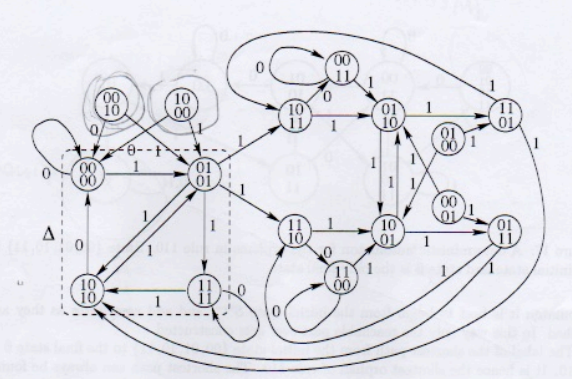
\includegraphics[width=.7\textwidth]{img/sistemi_complessi/automa_prodotto.png}
    \caption{Esempio di automa prodotto con la sua diagonale}
    \label{fig:automa_prodotto}
\end{figure}

\begin{teorema}
    Dato un automa CA monodimensionale allora \textbf{non è iniettivo} sse:
    \begin{enumerate}
        \item \label{cond:non_iniettiva_1} il suo grafo prodotto ha un ciclo che contiene un nodo fuori $\Delta$
        \item \label{cond:non_iniettiva_2}il suo grafo prodotto ha un ciclo che contiene un nodo in $\Delta$ e
              un nodo fuori $\Delta$
    \end{enumerate}
    \begin{proof}
        Dimostriamo i singoli punti:
        \begin{itemize}
            \item condizione \ref{cond:non_iniettiva_1}: se CA non è iniettivo
                  allora non è iniettivo sulle spazialmente periodiche. Quindi esisteranno
                  due configurazioni $c,e, c\ne e$ spazialmente periodiche tali che $F(c) = F(e)$,
                  quindi esisterà un camino sul grafo prodotto composto dai vertici che
                  rappresentano $c$ ed $e$. Il precedente cammino sarà composto da un ciclo
                  contenente nodi fuori dalla diagonale dal momento che $c\ne e$ per la
                  definizione di diagonale. Viceversa, dato un ciclo sul grafo prodotto contenente nodi
                  fuori dalla diagonale, allo questo significa che rappresenta due
                  configurazioni differenti aventi la stessa immagine, quindi CA non è
                  iniettivo.
            \item condizione \ref{cond:non_iniettiva_2}: Sia $q\in A$ arbitrario.
                  Se CA non è suriettivo allora significa che non è iniettivo sulle
                  configurazioni $q$-finite. Quindi esistono $c,e$ con $c\ne e $ configurazioni
                  $q$-finite tali che $F(c) =F(e)$. Il cammino corrispondente sul
                  grafo prodotto sarà composto da un ciclo all'interno di $\Delta$
                  seguito da un ciclo che esce da $\Delta$ per poi ritornare in $\Delta$.
                  Questo significa che il ciclo è composto da nodi sia nella diagonale,
                  sia fuori; quindi non è iniettivo. Viceversa, dato un ciclo composto da nodi nella diagonale
                  e fuori dalla diagonale, allora si ha un diamante, quindi CA non è suriettivo.
                  e fuori dalla diagonale, allora si ha un diamante, quindi CA non è suriettivo.

        \end{itemize}
    \end{proof}
\end{teorema}


Il grafo prodotto può essere ridotto rimuovendo alcune informazioni (figura \ref{fig:automa_prodotto_ridotto}):
\begin{itemize}
    \item tutti i nodi $v',v'' \in V\times V$ tali che $v'= (u,u'), v''=(u',u)$
          allora rappresentano le stesse configurazioni specchiate, quindi possono essere
          accorpati
    \item la diagonale può essere ridotta ad un unico nodo
\end{itemize}

\begin{figure}[!h]
    \centering
    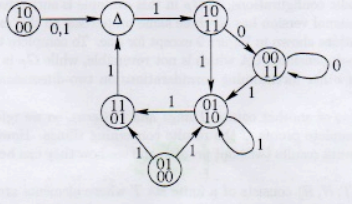
\includegraphics[width=.7\textwidth]{img/sistemi_complessi/automa_prodotto_ridotto.png}
    \caption{Esempio di automa prodotto ridotto}
    \label{fig:automa_prodotto_ridotto}
\end{figure}

Per scoprire se in un grafo ci sono dei cicli basta effettuare una DFS che ha una
complessità di $\mathcal{O}(|V|+|E|)$ e sapendo che $|V|= |V|^2$ dell'automa di
De Bruijn allora abbiamo un algoritmo polinomiale che ci permette di decidere
se il CA è suriettivo o iniettivo oppure no.

\subsection{Stabilità, instabilità e caos degli automi cellulari}
La notazione che verrà introdotto è valida per un qualsiasi \textbf{sistema dinamico a tempo
    discreto} (DTDS), ovvero per ogni $(X,F)$ dove $(X,d)$ è uno spazio metrico e
$F:X\rightarrow X$ è una trasformazione continua. Nel nostro caso $X \equiv A^\mathbb{Z}$,
$F$ è la regola globale e $d$ è la distanza di Tychonoff.

\begin{definizione} [\textbf{Punto di stabilità (equicontinuo, Lyapunov stable)}]
    % TODO: controllare not equal se va solo nelle definizioni di instabilità o anche in quelle di stabilità
    $x\in X$ è un \textbf{punto stabile} (equicontinuo, Lyapunov stable) sse
    $$\forall \epsilon > 0,\exists \delta > 0, \forall y\in X, d(y,x) < \delta \implies \forall t\in \mathbb{N} d(F^t(y),F^t(x))< \epsilon$$

    Con $X \equiv A^\mathbb{Z}$ e $d$ distanza di Tychonoff allora possiamo riscrivere
    la definizione in questo modo, $x\in X$ è un \textbf{punto stabile} sse
    $$\forall n\in \mathbb{N} ,\exists m\in \mathbb{N} , \forall y\in A^\mathbb{Z}, d(y,x) < \frac{1}{2^m} \implies \forall t\in \mathbb{N} d(F^t(y),F^t(x))< \frac{1}{2^n}$$
    Equivale a dire:
    $$\forall n\in \mathbb{N} ,\exists m\in \mathbb{N} , \forall y\in A^\mathbb{Z}, y_{[-m,m]} = x_{[-m,m]} \implies \forall t\in \mathbb{N} F^t(y)_{[-n,n]}=F^t(x)_{[-n,n]}$$
\end{definizione}
Questa coincide con la definizione di continuità con l'aggiunta del controllo che
sia continua anche sulle successive applicazioni, quindi per i successivi passi
temporali.

\begin{definizione} [\textbf{Punto di instabilità}]
    $x\in X$ è un \textbf{punto instabile} sse $x$ \textbf{non è stabile}

    $$\exists \epsilon > 0,\forall \delta > 0, \exists y\in X,x \ne y, d(y,x) < \delta \land \exists t\in \mathbb{N} d(F^t(y),F^t(x))\ge \epsilon$$
    Con $X \equiv A^\mathbb{Z}$ e $d$ distanza di Tychonoff allora possiamo riscrivere
    la definizione in questo modo,
    $$\exists n\in \mathbb{N} ,\forall m\in \mathbb{N} , \exists y\in A^\mathbb{Z},x \ne y, d(y,x) < \frac{1}{2^m} \land \exists t\in \mathbb{N} d(F^t(y),F^t(x))\ge \frac{1}{2^n}$$
    Equivale a dire:
    $$\exists n\in \mathbb{N} ,\forall m\in \mathbb{N} , \exists y\in A^\mathbb{Z},x \ne y, y_{[-m,m]} = x_{[-m,m]} \land \exists t\in \mathbb{N} F^t(y)_{[-n,n]}\ne F^t(x)_{[-n,n]}$$


\end{definizione}

\begin{definizione} [\textbf{Sistema stabile (stabilità globale)}]
    $(X,F)$ è \textbf{stabile} se $\forall x \in X$, $x$ è un \textbf{punto stabile}
\end{definizione}

\begin{definizione} [\textbf{Sistema equicontinuo (equicontinuità)}]
    $(X,F)$ è \textbf{equicontinuo} dove la definizione di stabilità di un punto cambia
    perché $\epsilon$ non dipende per un particolare punto $x\in X$ ovvero
    $$\forall \epsilon > 0,\exists \delta > 0, \forall y, x\in X, d(y,x) < \delta \implies \forall t\in \mathbb{N} d(F^t(y),F^t(x))< \epsilon$$
\end{definizione}

\begin{nota}
    L'equicontinuità è più stringente rispetto alla stabilità globale. Quando $X=A^\mathbb{Z}$
    si hanno due definizioni equivalenti e possono essere riscritte come
    $$\forall n\in \mathbb{N} ,\exists m\in \mathbb{N} , \forall y,x\in A^\mathbb{Z}, y_{[-m,m]} = x_{[-m,m]} \implies \forall t\in \mathbb{N} F^t(y)_{[-n,n]}=F^t(x)_{[-n,n]}$$
    $$\forall n\in \mathbb{N} ,\exists m\in \mathbb{N} , \forall y,x\in A^\mathbb{Z}, y_{[-m,m]} = x_{[-m,m]} \implies \forall t\in \mathbb{N} F^t(y)_{[-n,n]}=F^t(x)_{[-n,n]}$$
\end{nota}


\begin{definizione} [\textbf{Sistema instabile (instabilità globale)}]
    $(X,F)$ è \textbf{instabile} se $\forall x \in X$, $x$ è un \textbf{punto instabile}
\end{definizione}

\begin{definizione} [\textbf{Sistema sensibile alle condizioni iniziali (effetto butterfly)}]
    $(X,F)$ è \textbf{sensibile alle condizioni iniziali} se
    $$\exists \epsilon > 0,\forall x \in X, \forall \delta > 0, \exists y\in X,x \ne y, d(y,x) < \delta \land \exists t\in \mathbb{N} d(F^t(y),F^t(x))\ge \epsilon$$
    In $A^\mathbb{Z}$
    $$\exists n\in \mathbb{N} ,\forall x \in A^\mathbb{Z}, \forall m\in \mathbb{N} , \exists y\in A^\mathbb{Z},x \ne y, y_{[-m,m]} = x_{[-m,m]} \land \exists t\in \mathbb{N} F^t(y)_{[-n,n]}\ne F^t(x)_{[-n,n]}$$
\end{definizione}


\begin{nota}
    Un sistema sensibile è un sistema instabile in cui la constante $\epsilon$
    non dipende da $x\in X$, questa viene chiamata anche costante sensitiva ed
    non dipende da $x\in X$, questa viene chiamata anche costante sensitiva ed
    è una specifica feature del sistema.
\end{nota}


\begin{nota}
    Ricorda che nelle definizioni di punti e sistemi stabili, equicontinui, instabili e sensibili
    alle condizioni i coefficienti $m$ e $n$ sono relazionati nel seguente modo $m> n$.
    Questo è vero perché si applica $f^\ast$ su una configurazione lunga $m$, quindi
    ritorna una configurazione lunga $n$ più piccola.
\end{nota}

Se un punto di equicontinuità allora si ha che delle variazioni fuori da $[-m,m]$
non si propagheranno all'interno di $[-n,n]$.

Se un punto di instabilità allora si ha che delle variazioni fuori da $[-m,m]$
prima o poi si propagheranno all'interno di $[-n,n]$.

\begin{definizione}[\textbf{Residuale}]
    Sia $(X,d)$ uno spazio metrico. Dato $Y\subseteq X$, $Y$ è \textbf{residuale}
    se contiene un intersezione numerabile di insiemi aperti e densi di $X$.
\end{definizione}
\begin{esempio}
    Sia $\mathbb{I}$ l'insieme dei numeri irrazzionali, esso è definito come
    $\mathbb{I} =\bigcap_{q\in \mathbb{Q}} R-\{q\}$.
    Possiamo dire:
    \begin{itemize}
        \item $\mathbb{I}$ è denso in $\mathbb{R}$
        \item $\mathbb{R} - \{q\} = \left(-\infty, q\right)\cup \left(q,+\infty\right)$ è aperto.
        \item $\mathbb{R} - \{q\}$ è denso in $\mathbb{R}$
        \item $\bigcap_{q\in \mathbb{Q}} R-\{q\}$ è numerabile
    \end{itemize}
    $\mathbb{I}$ contiene un'intersezione numerabile di sottoinsiemi di $\mathbb{R}$ densi e aperti, quindi è residuale.
\end{esempio}

\begin{definizione}[\textbf{Almeno equicontinuo}]
    $(X,F)$ è \textbf{almeno equicontinuo} se l'insieme $\xi$ dei suoi punti di
    equicontinuità è \textbf{residuale}.
\end{definizione}
\begin{definizione}[\textbf{Punto ultimamente periodico}]
    $x\in X $ è \textbf{ultimamente periodico} se esistono due naturali $p_x>0$ (chiamato
    periodo) e $q_x\ge 0$ (chiamato preperiodo) tale che $F^{q_x+p_x} = F^{q_x}$, o
    equivalentemente,
    $$\forall x\in X,\exists p_x>0,q_x\ge 0:F^{q_x+p_x}(x) = F^{q_x}(x)$$.
    $$\forall x\in X,\exists p_x>0,q_x\ge 0:F^{q_x+p_x}(x) = F^{q_x}(x)$$.
\end{definizione}
\begin{definizione}[\textbf{Ultima periodicità del sistema}]
    $(X,F)$ è \textbf{ultimamente periodico} se esistono due naturali $p>0$ (chiamato
    periodo) e $q\ge 0$ (chiamato preperiodo) tale che $F^{q+p} = F^q$, equivalentemente,
    $$\forall x\in X,F^{q+p}(x) = F^q(x)$$
    $$\forall x\in X,F^{q+p}(x) = F^q(x)$$
\end{definizione}
Ultima periodicità significa che tutte le configurazioni dopo un numero di applicazioni
finite di $F$ (in totale $q$) (configurazione zero) diventano periodiche di periodo $p$ ovvero dopo
$p$ colpi di $F$ si torna alla configurazione zero.
$p$ colpi di $F$ si torna alla configurazione zero.

\begin{definizione} [\textbf{Nilpotenza}]
    \textbf{Nilpotenza} significa $\exists t:\forall x\in X$$F^t(x)$ sarà la configurazione
    zero.
\end{definizione}

\begin{nota}
    $\sigma(zero) = zero$ e $F(zero) = zero$ quindi $zero$ è anche un \textbf{punto fisso}.
    Inoltre:
    \begin{itemize}
        \item $\sigma(zero) = \sigma(F^t(x)) = F^t(\sigma(x)) = zero$
        \item $F(zero) = F(F^t(x)) = F^t(F(x)) = zero$
    \end{itemize}
    Quindi $zero$ è una configurazione composta da soli caratteri uguali.
\end{nota}

L'insieme di configurazioni $\{x,F(x), \dots, F^{q-1}(x)\}$ è chiamato transiente
e la sua lunghezza è $q$.

L'insieme di configurazioni $\{F^q(x), F^{q+1}(x), \dots, F^{q+p-1}(x)\}$ è chiamato ciclo
e la sua lunghezza è $p$.

\begin{nota}
    Sia $(X,F)$ con $|X|<\infty$, quindi un CA composto da configurazioni finite.

    $(X,F)$ è \textbf{ultimamente periodico} perché nell'esecuzione sull'CA le
    configurazioni saranno spazialmente periodiche perché
    $\forall x\in X\exists q_\ast \ge 0, p_\ast >0: F^{q_\ast +p_\ast}(x)=F^{q_\ast}(x)$.

    Se noi considerassimo $q=\max\{q_x|x\in X\}$ e $p=\text{mcd}\{p_x|x\in X\}$,
    innanzitutto sappiamo che i singoli insiemi sono finiti visto che le configurazioni
    sono finite e in aggiunta, $\forall x\in X:F^{q+p}(x)=F^{q}(x)$
    quindi il sistema sarà \textbf{ultimamente periodico}.
\end{nota}

Ecco perché non ha senso analizzare sistemi finiti, perché sarebbero ultimamente
periodici e quindi non possiamo studiare comportamenti instabili.

\begin{teorema}
    Sia $(X,F)$ un DTDS, allora:
    \begin{itemize}
        \item $(X,F)$ è ultimamente periodico $\implies$ $(X,F)$ equiconinuo (solo quando $(X,d)$ è compatto)
        \item $(X,F)$ è ultimamente periodico $\implies$ $(X,F)$ equiconinuo (solo quando $(X,d)$ è compatto)
        \item $(X,F)$ è equiconinuo $\implies$ $(X,F)$ almeno equicontinuo
    \end{itemize}
    \begin{proof}
        dimostriamo i singoli punti:
        \begin{itemize}
            \item U.P $\implies$ Equicontinuo: dobbiamo dimostrare la definizione
                  di equicontinuità.
                  $$\forall \epsilon > 0,\exists \delta > 0, \forall y, x\in X, d(y,x) < \delta \implies \forall t\in \mathbb{N} d(F^t(y),F^t(x))< \epsilon$$
                  Scelto arbitrariamente $\epsilon>0$ dal momento che $F^0, F^{1}, \dots, F^{q-1},F^{q},F^{q+1},\dots,F^{q+p-1}$
                  sono funzioni uniformamente continue allora applicando singolarmente le funzioni:
                  \begin{equation*}
                      \begin{array}{cl}
                          \left[F^0\right]       & \exists \delta_0 > 0, \forall y, x\in X, d(y,x) < \delta_0 \implies d(F^0(y),F^0(x))< \epsilon                         \\
                          \left[F^1\right]       & \exists \delta_1 > 0, \forall y, x\in X, d(y,x) < \delta_1 \implies d(F^1(y),F^1(x))< \epsilon                         \\
                          \vdots                 & \vdots                                                                                                                         \\
                          \left[F^q\right]       & \exists \delta_q > 0, \forall y, x\in X, d(y,x) < \delta_q \implies d(F^q(y),F^q(x))< \epsilon                         \\
                          \vdots                 & \vdots                                                                                                                         \\
                          \left[F^{q+p-1}\right] & \exists \delta_{q+p-1} > 0, \forall y, x\in X, d(y,x) < \delta_{q+p-1} \implies d(F^{q+p-1}(y),F^{q+p-1}(x))< \epsilon \\
                      \end{array}
                  \end{equation*}
                  allora $\exists \delta = \min \{\delta_0,\delta_1, \dots, \delta_q,\dots, \delta_{q+p-1}\}$ tale che
                  $$\forall y, x\in X, d(y,x) < \delta \implies \forall t\in \{0,1,\dots,q,\dots,q+p-1\} d(F^t(y),F^t(x))< \epsilon $$
                  $$\forall y, x\in X, d(y,x) < \delta \implies \forall t\in \{0,1,\dots,q,\dots,q+p-1\} d(F^t(y),F^t(x))< \epsilon $$
            \item Equiconinuo $\implies$ almeno equicontinuo: se $(X ,F)$ è equiconinuo
                allora $\xi = X$.  Abbiamo che $\xi = \bigcap_{n\in \mathbb{N}}X_n$ con $X_n= X$,
                dove $X$ è aperto e denso, quindi $(X,F)$ è almeno equicontinuo.
        \end{itemize}
    \end{proof}
\end{teorema}

\begin{nota}
    Una qualsiasi configurazione \textbf{spazialmente periodica} è \textbf{ultimamente periodica}.
    Sia $x\in A^\mathbb{Z}$ tale che $\sigma ^n(x)=x$ per un $n\in \mathbb{N}$.

    Sia $x=^\infty u^{(0)\infty}$ per qualche $u^{(0)}\in  A^n$ e sia $F$ una regola 
    globale di un CA. 

    Dal momento che un'immagine di una spazialmente periodica rimane spazialmente periodica,
    abbiamo:
    \begin{itemize}
        \item $F(x)=^\infty u^{(1)\infty}$ per qualche $u^{(1)}\in  A^n$
        \item $F(x)=^\infty u^{(2)\infty}$ per qualche $u^{(2)}\in  A^n$
        \item $\vdots$
        \item $F(x)=^\infty u^{(t)\infty}$ per qualche $u^{(t)}\in  A^n$
    \end{itemize}
    Dal momento che $A^n$ è finito, necessariamente $\exists q_x\ge 0, p_x> 0$ 
    Dal momento che $A^n$ è finito, necessariamente $\exists q_x\ge 0, p_x> 0$ 
    tale che $F^{q_x+p_x-1}(x)=F^{q_x}(x)$ ($x$ è ultimamente periodica).
\end{nota}
\begin{definizione}[\textbf{Blocking word}]
    Sia $u\in A^n$ per qualche $n\in \mathbb{N}$. Sia $s\in \mathbb{N}$ con $s>0$,
    la parola $u$ è $s$\textbf{-blocking} se $\exists \theta\in [0,n-s]$ (offset)
    tale che $\forall x,y\in A^\mathbb{Z}:x_{[0,n)}=y_{[0,n)}=u$ e vale $\forall t\in \mathbb{N}:
    tale che $\forall x,y\in A^\mathbb{Z}:x_{[0,n)}=y_{[0,n)}=u$ e vale $\forall t\in \mathbb{N}:
    F^t(x)_{[\theta,\theta +s)} =F^t(y)_{[\theta,\theta +s)}$
\end{definizione}

Se $s\ge r$ allora $u$ è un muro che impedisce alle celle a sinistra di influenzare 
l'evoluzione delle celle a destra, quindi $u$ produce una disconnessione dello 
spazio delle celle $\mathbb{Z}$. Tutto questo si può generalizzare facendo iniziare 
$u$ ad un indige $i$ generico, attenzione che si devono incrementare di conseguenza 
tutti gli indici.

\begin{nota}
    Ecco la generalizzazione delle parole bloccanti, $u$ è la parola colorata.
    \begin{figure}[!h]
        \centering
        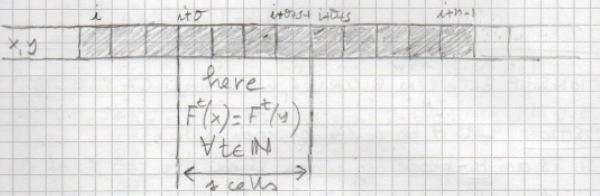
\includegraphics[width=.7\textwidth]{img/sistemi_complessi/parola_bloccante.png}
        \caption{Generalizzazione delle parole bloccanti che iniziano da $i$}
        \label{fig:parola_bloccante}
    \end{figure}
\end{nota}

\begin{nota}
    Se $u\in A^n$ è $s$-blocking allora ogni $v\in A^m$ con $m>n$ tale che ha 
    $u$ come sottosequenza allora anche $v$ è $s$-blocking.
\end{nota}

\begin{nota}
    Se $u\in A^n$ è $s_1$-blocking con un offset $\theta_1$ e $v\in A^m$ è  $s_2$-blocking
    con un offset $\theta_2$, allora $\forall w \in A^+$ la parola $uwv$ è una parola 
    bloccante. 
    La regione che va da $\theta_1$ a $s_2$ sarà lunga $n - \theta_1 + | w | + \theta_2 + s_2$.
    \begin{figure}[!h]
        \centering
        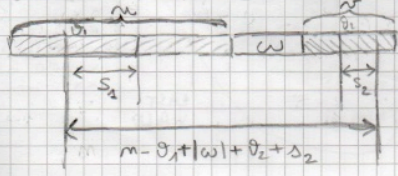
\includegraphics[width=0.5\textwidth]{img/sistemi_complessi/blocking_word_1.png}
    \end{figure}
    \begin{figure}[!h]
        \centering
        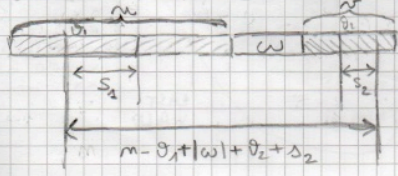
\includegraphics[width=0.5\textwidth]{img/sistemi_complessi/blocking_word_1.png}
    \end{figure}
\end{nota}

Le parole bloccanti sono in relazione con la stabilità degli automi cellulari.
\begin{teorema}
    Sia $F$ la regola globale per un CA di raggio $r$. Se $u$ è una parola $r$-bloccante
    allora l'insieme $\xi$ dei punti di equicontinuità di $F$ è infinito (e denso).
    \begin{proof}
        Sia $x\in A^\mathbb{Z}$ una qualsiasi configurazione del tipo $(uA^\ast)^+$,
        andremo a dismostrare che $x$ sia un punto di equicontinuità, ovvero 
        $$\forall n\in \mathbb{N} ,\exists m\in \mathbb{N} , \forall y\in A^\mathbb{Z}, y_{[-m,m]} = x_{[-m,m]} \implies \forall t\in \mathbb{N} F^t(y)_{[-n,n]}=F^t(x)_{[-n,n]}$$
        Scelto un $n \in \mathbb{N}$ e sia $m$ tale che $[-n,n]\subseteq [-m,m]$
        Scelto un $n \in \mathbb{N}$ e sia $m$ tale che $[-n,n]\subseteq [-m,m]$
        e $[-n,n]$ è contenuto all'interno del segmento $[-m,m]$ tale che 
        inizi all'interno segmento definito dal primo muro della prima occorrenza di $u$ in $[-m,m]$ fino 
        all'ultimo muro dell'ultima occorrenza di $u$. Allora $x$ è un punto di 
        equicontinuità. Questo deriva dal fatto che $u$ è $r$-bloccante, quindi un
        qualsiasi cambiamento esterno a $[-m,m]$ non influenza la regione interna
        delimitata dalla parola $u$.
        \begin{figure}[!h]
            \centering
            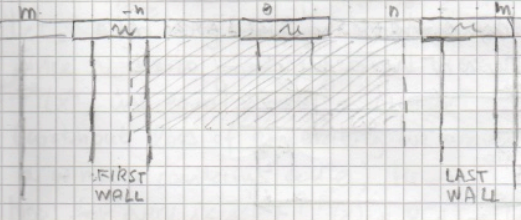
\includegraphics[width=0.5\textwidth]{img/sistemi_complessi/blocking_word_2.png}
        \end{figure}
        \begin{figure}[!h]
            \centering
            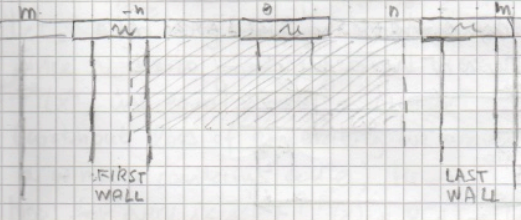
\includegraphics[width=0.5\textwidth]{img/sistemi_complessi/blocking_word_2.png}
        \end{figure}
    \end{proof} 
\end{teorema}
\begin{teorema}[\textbf{Caratterizzazzione della equiconinuità}]
    Sia $\langle A,r,f\rangle$ un CA e sia $F$ la regola globale allora i seguenti
    punti sono equivalenti:
    \begin{enumerate}
        \item \label{cond:non_carr_equi_1} $(A^\mathbb{Z}, F)$ è un \textbf{sistema equicontinuo}
        \item \label{cond:non_carr_equi_2} $\exists k>0$ tale che $\forall u \in A^{2k+1}$, $u$ è $r$-bloccante
        \item \label{cond:non_carr_equi_3} $(A^\mathbb{Z}, F)$ è \textbf{ultimamente periodico}
    \end{enumerate}
    \begin{proof}[dimostrazione opzionale]
        Dimostriamo le singole implicazioni:
        \begin{itemize}
            \item \ref{cond:non_carr_equi_1} $\implies $\ref{cond:non_carr_equi_2}:
            Sappiamo che il sistema è equicontinuo, quindi
            $$\forall n\in \mathbb{N} ,\exists k\in \mathbb{N} , \forall y,x\in A^\mathbb{Z}, y_{[-k,k]} = x_{[-k,k]} \implies \forall t\in \mathbb{N} F^t(y)_{[-n,n]}=F^t(x)_{[-n,n]}$$
            Sia $n=r$ allora 
            $$\exists k\in \mathbb{N} , \forall y,x\in A^\mathbb{Z}, y_{[-k,k]} = x_{[-k,k]} \implies \forall t\in \mathbb{N} F^t(y)_{[-r,r]}=F^t(x)_{[-r,r]}$$
            Pertanto sappiamo che esistono parole $r$-bloccanti e presa una qualsiasi $u\in A^{2k+1}$ è $r$-bloccante per definizione.
            \item \ref{cond:non_carr_equi_2} $\implies $\ref{cond:non_carr_equi_3}: 
            andremo a mostrare che esistono $p>0$ e $q\ge 0$ tali che $F^{q+p} = F^q$.
            Per ogni $u\in A^{2k+1}$, consideriamo $x^{(u)}=^\infty u^\infty$ (per 
            definizione è spazialmentente periodica e per ipotesi $r$-bloccante).
            Sappiamo che $\{F^t(x^{(u)})\}_{t\in \mathbb{N}}$ è ultimamente periodica,
            allora  anche $\{F^t(x^{(u)})_0\}_{t\in \mathbb{N}}$ è ultimamente periodica.
            Sappiamo che $\{F^t(x^{(u)})\}_{t\in \mathbb{N}}$ è ultimamente periodica,
            allora  anche $\{F^t(x^{(u)})_0\}_{t\in \mathbb{N}}$ è ultimamente periodica.
            Questo significa che $\exists p_u>0$ e $q_u\ge 0$ tali che $F^{q_u+p_u}(x^{(u)})_0 =F^{q_u}(x^{(u)})_0 $.
            Sia $p=\text{mcd}\{p_u|u\in A^{2k+1}\}$ e $q=\max\{q_u|u\in A^{2k+1}\}$.
            Allora $\forall u\in A^{2k+1}, F^{q+p}(x^{(u)})_0 = F^{q}(x^{(u)})_0$.

            Sia $x\in A^\mathbb{Z}$ una qualsiasi configurazione e $u=x_{[-k,k]}$.
            Dal momento che $u$ è $r$-bloccante, $\forall t\in \mathbb{N}, F^t(x)$
             e $ F^t(x^{(u)})$ sono uguali per una finestra diu lunghezza $r$, 
             senza perdere d igeneralità supponiamo che contenga la cella $0$, allora 
             $F^{q+p}(x)_0 = F^{q}(x)_0$. Ora $\forall i\in \mathbb{Z}$
             $$F^{q+p}(x)_i = \sigma^i(F^{q+p}(x))_0 = F^{q+p}(\sigma^i(x))_0= F^{q}(\sigma^i(x))_0 = \sigma^i(F^{q}(x))_0 = F^{q}(x)_i$$

            \item \ref{cond:non_carr_equi_3} $\implies $\ref{cond:non_carr_equi_1}: 
            è già stata dimostrata.
        \end{itemize}
    \end{proof}
\end{teorema}
Se si negano le condizioni si ha la caratterizzazione per i sistemi sensibili
alle condizioni iniziali.

\begin{nota}
    Se il sistema è \textbf{equicontinuo} allora tutte le parole da un certo punto 
    in poi sono bloccanti, mentre se è \textbf{almeno equicontinuo} allora ne esisterà
    una che prima o poi diventerà bloccante.
\end{nota}

\begin{teorema}[\textbf{Caratterizzazzione dell'almeno equiconinuità}]
\begin{teorema}[\textbf{Caratterizzazzione dell'almeno equiconinuità}]
    Sia $\langle A,r,f\rangle$ un CA e sia $F$ la regola globale allora i seguenti
    punti sono equivalenti:
    \begin{enumerate}
        \item \label{cond:non_carr_a_equi_1} $(A^\mathbb{Z}, F)$ non è \textbf{sistema 
        sensibile alle condizioni iniziali}
        \item \label{cond:non_carr_a_equi_2} $(A^\mathbb{Z}, F)$ ha una parola $r$-bloccante
        \item \label{cond:non_carr_a_equi_3} $(A^\mathbb{Z}, F)$ è \textbf{almeno equiconinuo}
    \end{enumerate}
    \begin{proof}
        Dimostriamo le singole implicazioni:
        \begin{itemize}
            \item \ref{cond:non_carr_equi_1} $\implies $\ref{cond:non_carr_equi_2}:
            per ipotesi il sistema non è sensibile alle condizioni iniziali quindi
            $$\forall n\in \mathbb{N} ,\exists x \in A^\mathbb{Z}, \exists m\in \mathbb{N} , \forall y\in A^\mathbb{Z}, y_{[-m,m]} = x_{[-m,m]} \implies \forall t\in \mathbb{N} F^t(y)_{[-n,n]}= F^t(x)_{[-n,n]}$$
            Scegliamo arbitrariamente $n$ in modo tale che $2n+1\ge r$.
            $$\exists x \in A^\mathbb{Z}, \exists m\in \mathbb{N} , \forall y\in A^\mathbb{Z}, y_{[-m,m]} = x_{[-m,m]} \implies \forall t\in \mathbb{N} F^t(y)_{[-n,n]}= F^t(x)_{[-n,n]}$$
            Quindi $u=x_{[-m,m]}$ è $(2n+1)$-bloccante quindi
            $$\forall z,z'\in A^\mathbb{Z}: z_{[-m,m]}=z'_{[-m,m]} = x_{[-m,m]} =u$$
            Questo significa che 
            $$\forall t, F^t(z)_{[-n,n]} = F^t(x)_{[-n,n]}\text{ e } F^t(z')_{[-n,n]} = F^t(x)_{[-n,n]}$$
            Quindi $F^t(z)_{[-n,n]} = F^t(z')_{[-n,n]},\forall t$. In conclusione $u$
            è anche $r$-bloccante da $2n+1\ge r$.
            \item \ref{cond:non_carr_equi_2} $\implies $\ref{cond:non_carr_equi_3}: 
            abbiamo già dimostrata.
            \item \ref{cond:non_carr_equi_3} $\implies $\ref{cond:non_carr_equi_1}: 
            se il sistema è A.E. allora esiste un punto di equicontinuità e quindi
            non può essere sensibile alle condizioni iniziali.
        \end{itemize}
    \end{proof}
\end{teorema}

\begin{teorema}
    Sia $\langle A,r,f\rangle$ un CA, è decidibile stabilire se data una word $u\in A^+$
    è $r$-bloccante
\end{teorema}

\begin{teorema}
    Il problema di stabilire se il CA ammette una parola $r$-bloccante 
    è indecidibile.
\end{teorema}

\begin{teorema}
    Stabilire se un CA è almeno equicontinuo o sensibile alle condizioni iniziali 
    è un problema indecidibile.
\end{teorema}

\begin{teorema}
    Stabilire se un CA è nilpotente è un problema indecidibile.
\end{teorema}

\begin{teorema}
    Stabilire se un CA è equicontinuo (o ultimamente periodico) è un problema indecidibile.
    \begin{proof} [cenni di dimostrazione]
        Per assurdo assumiamo che l'ultima periodicità è decidibile. Sia 
        $\langle A,r,f\rangle$  un CA e $F$ la sua regola globale, dal momento
        che l'ultima periodicità è decidibile, possiamo stabilire quando $F$ entra 
        nei seguenti casi:
        \begin{itemize}
            \item $F$ non è ultimamente periodica $\implies$ $F$ non è nilpotente
            \item $F$ è ultimamente periodica allora $\exists p>0, q\in \mathbb{N}$
            tale che $F^q=F^{q+p}$. Dalle configurazioni spazialmente periodiche,
            $p$ e $q$ sono computabili quindi:
            \begin{itemize}
                \item $p\ne 1\implies F$ non è nilpotente
                \item $p= 1$ allora:
                \begin{itemize}
                    \item Se $^\infty q^\infty$ è l'unica $x$ tale che $F(x)=x$ allora
                    $F$ è nilpotente
                    \item Altrimenti $F$ non è nilpotente
                \end{itemize}
            \end{itemize}
        \end{itemize}
    \end{proof}
\end{teorema}

\begin{definizione}[\textbf{Permutativa RM/LM}]
    $f:A^{2r+1}\rightarrow A$ è \textbf{permutativa} se 
    $$\forall b\in A, \forall u \in A^{2r}, \exists ! a\in A: f(ua)=b \ (f(au)=b)$$
    Permutativa perché $\forall u \in A^{2r}, f_{|u}:A\rightarrow A:f_{|u}(a) = b$
    e $f_{|u}$ è biettiva.
\end{definizione}

\begin{teorema}
    Stabilire se una regola locale è permutativa è un problema decidibile.
\end{teorema}

\begin{nota}
    Le regole locali possono essere:
    \begin{itemize}
        \item solo LM permutive
        \item solo RM permutive
        \item sia LM sia RM permutive
    \end{itemize}
\end{nota}

\begin{teorema}
    Se $f$ è una regola locale RM o LM permutive allora la regola globale del CA 
    $F$ è suriettiva.
    \begin{proof}
        Dobbiamo mostrare che la regola globale sia suriettiva, questo significa
        che dobbiamo dimostrare che la regola globale sia bilanciata ovvero
        $$\forall v \in A^+, |f^{-1}(v)| = |A|^{2r}$$
        Scelto arbitrariamente $v\in A^n$ e sia $u\in A^{2r}$ una qualsiasi parola.
        
        Supponiamo che $f$ sia $RM$, allora dato $v$ possiamo ottenere tutte le parole
        appartenenti all'insieme $f^{-1}(v)$ nel seguente modo, dato un carattere
        in posizione $v_i$, dal momento che $f$ è RM allora quello coincide col
        carattere della configurazione di partenza alla posizione $i+r$. Quindi 
        $v$ sarà la sottoconfigurazione di partenza che comparirà più a destra,
        mentre $u$ sarà la stringa che rimane da aggiungere a $v$ per riottenere $v$.
        Quindi $u$ può essere composta da un totale di $|A|^{2r}$ possibili scelte 
        di caratteri e questo coincide con la cardinalità delle preimmagini di $v$.
        Quindi $f$ è bilanciata.
        \begin{figure}[!h]
            \centering
            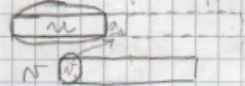
\includegraphics[width=.3\textwidth]{img/sistemi_complessi/preimmagini.png}
        \end{figure}
    \end{proof}
\end{teorema}

\begin{teorema}
    Se $F$ un CA con una regola locale $f:A^{2r+1}\rightarrow A$. $\forall t\in \mathbb{N}$
    sia $f^{(t)}:A^{2rt+1}\rightarrow A$ la regola locale di un CA $F^t$. Se $f$
    è RM/LM permutativa allora anche $f^{(t)}$ lo è.
\end{teorema}

\begin{nota}
    Se $F$ un CA con una regola locale $f$ L/R permutativa. Allora $F$ è sensibile 
    alle condizioni iniziali
    \begin{proof}
        Dovremo rincondurci alla definizione di sensibilità alle condizioni iniziali
        $\exists n=r: \forall x\in A^\mathbb{Z}, \forall m\in \mathbb{N},
        \exists y \in A^\mathbb{Z}, y\ne x, \text{ t.c. } y_{[-m,m]} = x_{[-m,m]}\land 
        \exists t\in \mathbb{N},F^t(y)_{[-r,r]} \ne F^t(x)_{[-r,r]}$.
        \exists t\in \mathbb{N},F^t(y)_{[-r,r]} \ne F^t(x)_{[-r,r]}$.

        Scelto arbitrariamente $x\in A^\mathbb{Z}$ e $m\in \mathbb{N}$ costruiamo
        $y\in A^\mathbb{Z}$ nel seguente modo: sia $t\in\mathbb{N}$ tale che 
        $[-m,m]\subset [r-tr,r+tr]$ e che:
        \begin{itemize}
            \item $y_{[r-tr, r+tr-1]} = x_{[r-tr, r+tr-1]}$, quindi $y_{[-m,m]} = x_{[-m,m]}$
            \item $y_{r+tr} \ne x_{r+tr}$
        \end{itemize} 
        Quindi $x$ e $y$ sono uguali da $-r-tr$ fino a $r+tr-1$, l'ultima cella 
        deve essere differente per le due stringhe.

        Essendo $f^{(t)}$ $R$-permutativa, allora secondo le due condizioni 
        specificate precedentemente allora 
        $$F^t(y)_r=f^{(t)}(y_{[r-tr, r+tr]})=f^{(t)}(y_{[r-tr, r+tr-1]}y_{r+tr})=$$
        $$=f^{(t)}(x_{[r-tr, r+tr-1]}y_{r+tr})$$
        $$F^t(x)_r=f^{(t)}(x_{[r-tr, r+tr-1]}x_{r+tr}) $$
        Questo significa che $F^t(y)_r \ne F^t(x)_r$.
    \end{proof}
\end{nota}

\begin{definizione}[(\textbf{Positivamente espansivo})]
    Un DTDS $(X,F)$ è detto \textbf{positivamente espansivo} se 
    $$\exists \epsilon >0, \forall x,y\in X, x\ne y, \exists t\in \mathbb{N}, d(F^t(y),F^t(x))\ge \epsilon$$
    Negli automi cellulari si ha
    $$\exists n\in \mathbb{N}, \forall x,y\in A^\mathbb{Z}, x\ne y, \exists t\in \mathbb{N}, F^t(y)_{[-n,n]} \ne F^t(x)_{[-n,n]}$$
    $$\exists n\in \mathbb{N}, \forall x,y\in A^\mathbb{Z}, x\ne y, \exists t\in \mathbb{N}, F^t(y)_{[-n,n]} \ne F^t(x)_{[-n,n]}$$
\end{definizione}

\begin{teorema}
    Sia $(X,F)$ un DTDS con $|X|=\infty$, se è espansivo allora è sensibile alle condizioni iniziali.

    Nel momento in cui avessi $|X|<\infty$ non sarebbe più sensibile perché posso
    prendere un intorno talmente piccolo da non avere altri alementi dal di fuori 
    dello stesso, portando ad non avere un sistema sensibile. 
\end{teorema}

\begin{nota}
    Se $(X,F)$ un DTDS con $|X|<\infty$ allora:
    \begin{enumerate}
        \item è ultimamente periodico, quindi equicontinuo
        \item è espansivo
    \end{enumerate}
    \begin{proof}
        Si può fare una bozza di dimostrazione del secondo punto.

        Sia $\epsilon = \min\{d(x,y)|x,y\in X, x\ne y\}$, sicuramente esiste un 
        elemento e dato che è una distanza allora sarà anche positiva non nulla.
        Per costruzione abbiamo $\forall x,y\in X, d(x,y)\ge \epsilon$, quindi il 
        sistema è espansivo e questo non vuol dire che $F$ sia instabile.
    \end{proof}
\end{nota}

\begin{teorema}
    Sia $(A^\mathbb{Z}, F)$ un CA con una regola locale  che sia LM sia RM permutive.
    Allora $F$ è posivamente espansivo.    
\end{teorema}

\begin{esempio}
    Data la regola locale $170$ (shift a sx), la regola è RM permutive, $F$ è positivamente espansivo.
    Data la regola locale $170$ (shift a sx), la regola è RM permutive, $F$ è positivamente espansivo.
    La stessa cosa vale per la regola del traffico ($184$).
\end{esempio}

La sensitività rispetto alle condizioni iniziali non è abbastanza per dire che un
sistema è anche \textbf{caotico}.

\begin{esempio}
    Supponiamo il seguente sistema $(X:=\mathbb{R},F(x):= 2\cdot x)$, una ipotetica
    evoluzione dinamica è $2^t\cdot x$.

    Quindi $\forall x,y\in X, d(F^t(x),F^t(y)) = |2^tx-2^ty|= 2^t|x-y|$. Si riesce 
    facilmente a dimostrare che il sistema è espansivo e sensibile alle condizioni 
    iniziali. Il problema è che noi non vogliamo considerare questo sistema caotico 
    iniziali. Il problema è che noi non vogliamo considerare questo sistema caotico 
    quindi dobbiamo introdurre nuovi concetti.
\end{esempio}

\begin{definizione}[\textbf{Transitivo}]
    Dato un DTDS $(X,F)$ è detto \textbf{transitivo} se 
    $$\forall x\in X,\forall \delta >0, \forall y\in X,\forall \epsilon>0, \exists 
    z\in X, d(z,x)< \delta \land \exists t\in \mathbb{N},d(F^t(z),y)<\epsilon$$

    In $(A^\mathbb{Z},F)$
    $$\forall x\in A^\mathbb{Z},\forall m \in\mathbb{N}, \forall y\in A^\mathbb{Z},\forall n\in\mathbb{N}, \exists 
    z\in A^\mathbb{Z}, z_{[-m,m]} = x_{[-m,m]} \land \exists t\in \mathbb{N},F^t(z)_{[-n,n]} = y_{[-n,n]}$$

\end{definizione}
Un sistema è transitivo se per ogni coppia di elementi, presi due loro vicini allora 
da un vicino si può raggiungere il secondo vicino in $t$ colpi di $F$. La proprietà 
di transitività specifica che il sistema deve essere irriducibile o non decomponibile

\begin{nota}
    La proprietà di transitività coincide con la proprietà di raggiungibilità debole.
\end{nota}

\begin{esempio}
    Il sistema lineare $F(x):= 2x$ non è transitivo perché dati $x=2$ e $y=-2$ 
    non esistono due elementi vicini raggiungibili visto che sono discordi.
\end{esempio}

\begin{definizione}[\textbf{Punto periodico}]
    $p\in X$ è un \textbf{punto periodico} se è ultimamente periodico di preperiodo
    $0$
\end{definizione}

\begin{definizione} [\textbf{Orbite densamente periodiche}]
    Dato un DTDS $(X,F)$ ha \textbf{Orbite densamente periodiche} (DPO) se
    $\forall x\in X, \forall \epsilon>0 \exists p \text{ punto periodico }:  d(x,p)<\epsilon$. 

    Quindi tutti gli elementi devono avere un elemento periodico vicino
\end{definizione}

\begin{esempio}
    Riprendendo l'esempio del sistema lineare, l'unico punto periodico è la configurazione $0$.
\end{esempio}
\begin{teorema}
    Dato un automa cellulare $(A^\mathbb{Z},F)$ allora:
    \begin{itemize}
        \item se è transitivo $\implies$ anche suriettivo
        \item se ha DPO $\implies$ anche suriettivo
    \end{itemize}
\end{teorema}

\begin{definizione} [\textbf{DTDS caotico}]
    Un DTDS $(X,F)$ è \textbf{caotico} se:
    \begin{itemize}
        \item $|X|=\infty$ 
        \item $(X,F)$ è \textbf{sensibile alle condizioni iniziali}
        \item $(X,F)$ è \textbf{transitivo}
        \item $(X,F)$ è \textbf{DPO}
    \end{itemize}
\end{definizione}

\begin{teorema}
    Se un DTDS $(X,F)$ con $|X|=\infty$ è transitivo e ha dei DPO allora è anche 
    sensibile alle condizioni iniziali. 
\end{teorema}

\begin{teorema} [\textbf{Solo per CA}]
    Se un CA $(A^\mathbb{Z},F)$ è transitivo allora è anche sensibile alle condizioni iniziali.
    Se un CA $(A^\mathbb{Z},F)$ è espansivo allora è anche transitivo.
\end{teorema}

Quindi per sapere se i CA sono caotici, le condizioni di $|X|=\infty$ e di sensibilità sono superflue,
basta solo controllare che sia transitivo e DPO.
Quindi per sapere se i CA sono caotici, le condizioni di $|X|=\infty$ e di sensibilità sono superflue,
basta solo controllare che sia transitivo e DPO.

\begin{teorema}
    Se un CA $(A^\mathbb{Z},F)$ con una regola locale LM/RM è transitivo e ha DPO.
\end{teorema}
\begin{teorema}
    Se un CA $(A^\mathbb{Z},F)$ con una regola locale LM/RM è caotico.
\end{teorema}

Ecco la classificazione finale degli automi cellulari (figura \ref{fig:classificazione_ca}).

\begin{figure}[!hb]
    \centering
    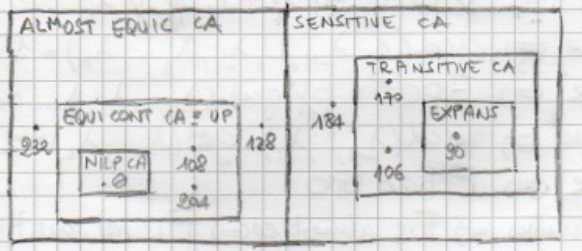
\includegraphics[width=0.5\textwidth]{img/sistemi_complessi/classificazione_ca.png}
    \caption{Classificazione automi cellulari}
    \label{fig:classificazione_ca}
\end{figure}

\begin{nota}
    Tutti i CA caotici studiati sono suriettivi ma non è detto che suriettività 
    implica caotico.
\end{nota}

\begin{nota}
    Esistono CA non permutivi che sono transitivi ed espansivi.

    Preso un qualunque L-permutive CA $F$ e un CA iniettivo $G$ che non è ne L ne R-permutive.
    Allora $G^{-1}\odot F\odot G$ è un CA che non è permutivo ma transitivo.
\end{nota}

In generale tutte le proprietà basate su un colpo di $F$ sono decidibili, mentre 
tutte le proprietà basate su $F^t$ sono indecidibili. L'unica proprietà basata 
su $F^t$ di cui non è stata dimostrata la sua indecidibilità è l'\textbf{espansivo},
ovvero non esiste un algoritmo che mi dica subito un CA è espansivo o no. In ogni 
caso si può credere che sia indecidibile.

\subsection{Automi cellulari lineari}
Definiamo $A= \mathbb{Z}_s = \{0,1,\dots, s-1\} =\mathbb{Z}/s\mathbb{Z}$ come 
l'insieme delle classi di equivalenza della relazione di equivalenza modulo $s$.
Sulla relazione di equivalenza si definisce un anello commutativo $\langle \mathbb{Z}_s,
+, \cdot \rangle$.

\begin{definizione} [\textbf{Regola locale lineare}]
    Sia $f:\mathbb{Z}_s^{2r+1}\rightarrow \mathbb{Z}_s$ è una \textbf{regola locale lineare} se  $\exists \lambda_{-r},
    \dots,\lambda_0,\dots,\lambda_r\in \mathbb{Z}_s$ tale che 
    \begin{equation*}
    \forall (x_{-r},\dots, x_r)\in \mathbb{Z}_s^{2r+1}, f(x_{-r},\dots, x_r) = \left(\sum_{i=-r}^{r}\lambda_ix_i\right)\mod s
    \end{equation*}
\end{definizione}

\begin{definizione} [\textbf{Automa cellulare lineare}]
    Un CA $F$ è lineare se è definito da una \textbf{regola locale lineare}.
\end{definizione}

Gli automi cellulari lineari sono utili perché su qualsiasi dimensione le proprietà
sono tutte decidibili, dal momento che ciascuna è caratterizzabile usando i divisori.

Ovviamente se $f$ è lineare allora $F$ è additiva e gli LCA sono utili per rappresentare 
sistemi che rispettano il principio di sovrapposizione, proprio come la maggior parte 
dei fenomeni reali.

\begin{teorema}
    Sia $(\mathbb{Z}_s^\mathbb{Z}, F)$ un LCA definito da una regola locale con i 
    seguenti coefficienti: $\lambda_{-r}, \dots,\lambda_0,\dots,\lambda_r$.

    Sia $\mathcal{P}$ che denota l'insieme dei fattori primi di $s$, denotiamo $a|b$
    il fatto che $a$ divide $b$, allora:
    \begin{itemize}
        \item $F$ è \textbf{suriettiva} $\iff\text{ MCD }(s,\lambda_{-r}, \dots,\lambda_0,\dots,\lambda_r) = 1$
        \item $F$ è \textbf{iniettiva} $\iff \forall p\in \mathcal{P}, \exists !\lambda_i: p\not |\lambda_i$
        \item $F$ è \textbf{transitivo} $\iff\text{ MCD }(s,\lambda_{-r}, \dots,\lambda_{-1},\lambda_{1},\dots,\lambda_r) = 1$
        \item $F$ è \textbf{sensibile alle condizioni iniziali} $\iff \exists  p\in \mathcal{P}: p\not |\text{ MCD }(\lambda_{-r}, \dots,\lambda_{-1},\lambda_{1},\dots,\lambda_r) $
        \item $F$ è \textbf{espansivo} $\iff \text{ MCD }(\lambda_{-r}, \dots,\lambda_{-1})=\text{ MCD }(\lambda_{1},\dots,\lambda_r)=1 $
        \item $F$ è \textbf{suriettiva} $\iff F$ ha DPO
        \item $F$ è \textbf{equiconinua} $\iff F$ è \textbf{almeno equiconinua} $\iff F$ non è \textbf{sensibile alle condizioni iniziali}
        \item $F$ è \textbf{caotica} $\iff F$ è \textbf{transitiva}
    \end{itemize}
\end{teorema}

\begin{teorema}
    Ciascuna proprietà è decidibile nei LCA.
\end{teorema}

\subsection{Automi cellulari $d$-D}
Dato un insieme di stati finito $S$.

\begin{definizione}[\textbf{Configurazioni}]
    Le \textbf{configurazioni} del CA sono elementi di $S^{\mathbb{Z}^d}$, ovvero
    funzioni che assegnano uno stato ad una particolare posizione $\mathbb{Z}^d\rightarrow S$.
\end{definizione}

Abbiamo che la singola cella non è nient'altro che un vettore nello spazio di dimensione 
$d$ che assume degli stati nell'insieme $S$.

\begin{definizione}[\textbf{Vettore di vicinanza}]
    Il \textbf{vettore di vicinanza} è un vettore di $n$ diversi vettori di $\mathbb{Z}^d$
    che specificano il relativo offsets di tutti gli elementi che specifica il 
    vicinato.
    $$N=\left(\underline{x_1},\underline{x_2},\dots,\underline{x_n}\right)$$
\end{definizione}

La cella vicina ad una cella $\underline{x }\in \mathbb{Z}^d$ è una qualsiasi cella $\underline{x}+\underline{x_i}$ 
con $\underline{x_i} \in N$.

\begin{esempio}
    Un esempio di vicinato in 2D per le due classiche regole di vicinato sono 
    le seguenti:
    \begin{itemize}
        \item \textbf{Von Neumann}: Il vicinato sono le celle che condividono un 
        lato
        $$N=\left(\left(0,0\right),\left(\pm 1,0\right), \left(0,\pm 1\right)\right)$$
        \item \textbf{Moore}: Il vicinato sono le celle che condividono un 
        lato e un vertice
        $$N=\{-1,0,1\}^2$$
    \end{itemize}
\end{esempio}

\begin{definizione}[\textbf{Regola locale}]
    La \textbf{regola locale} è una funzione 
    $$f:S^n\rightarrow S$$
    dove $n$ è la dimensione del vicinato $N$ ($n=|N|$) e il nuovo stato sarà
    $$f(a_1,\dots,a_n)$$
\end{definizione}

\begin{definizione}[\textbf{Regola globale}]
    La regola locale determina la dinamica globale del CA. Data una generica 
    configurazione $c$, diventa la nuova configurazione $e$ nel seguente modo:
    $$e(\underline{x}) = f(c(\underline{x}+ \underline{x}_1),c(\underline{x}+ \underline{x}_2),\dots, c(\underline{x}+ \underline{x}_n)), \forall \underline{x}\in \mathbb{Z}^d, \forall \underline{x}_i\in N$$
    Il passaggio dalla configurazione $c$ nella configurazione $e$ è scrivibile 
    formalmente nell'applicazione della \textbf{regola globale}
    $$G:S^{\mathbb{Z}^d}\rightarrow S^{\mathbb{Z}^d} $$
    tale che $G(c) = e$.
\end{definizione}

La generalizzazione della mappa shift al caso $d$-dimensionale non è altro che una 
traslazione $\tau$ determinata dal vettore $\underline{r}\in  \mathbb{Z}^d$, è
la trasformazione
$$\tau_{\underline{r}} :  S^{\mathbb{Z}^d} \rightarrow  S^{\mathbb{Z}^d}$$
$$\tau_{\underline{r}} :  S^{\mathbb{Z}^d} \rightarrow  S^{\mathbb{Z}^d}$$
tale che 
$$e =\tau_{\underline{r}}(c) \iff e(\underline{x}) =  c(\underline{x}+\underline{r}), \forall \underline{x},\underline{r}\in \mathbb{Z}^d$$

Un generico vettore $\underline{r}$ associato alla traslazione è un vettore 
unitario.

\begin{teorema} [\textbf{Hedlund}] 
    Sia $G:A^\mathbb{Z}\rightarrow A^\mathbb{Z}$ una qualunque funzione.
    $G$ è la regola globale di un CA \textbf{sse} entrambe le seguenti affermazioni
    sono vere:
    \begin{itemize}
        \item $G$ continua
        \item $G$ commuta con tutte le traslazioni
        \item $G$ commuta con tutte le traslazioni
    \end{itemize}
\end{teorema}

\begin{definizione} [\textbf{CA iniettivi, suriettivi e biettivi}]
    Un CA è chiamato:
    \begin{itemize}
        \item \textbf{iniettivo} se $G$ è inivettiva
        \item \textbf{suriettivo} se $G$ è suriettiva
        \item \textbf{biettivo} se $G$ è sia iniettiva, sia suriettiva
    \end{itemize}

\end{definizione}


\begin{definizione} [\textbf{CA reversivile}]
    Un CA è chiamato \textbf{reversibile} se esiste un altro CA con una funzione 
    globale $F$ che è l'inversa di un automa dato con funzione $G$, ovvero
    $$ G\odot F= F\odot G = Id$$
    Quindi $F$ e $G$ sono RCA e vengono chiamati \textbf{automi inversi}.
\end{definizione}

\begin{teorema}
    Un CA $G$ è reversibile sse è biettivo
\end{teorema}

\begin{definizione} [\textbf{Regola locale bilanciata}]
    Una \textbf{regola locale bilanciata} è una regola $f$ di un generico automa 
    tale che 
    $$|f^{-1}(a)| = | S | ^{n-1}, \forall a \in S$$
    Dove $S$ è l'insieme degli stati ($\mathbb{Z}^d$) e $n$ è la dimensione del 
    vicinato ($n=|N|$)
\end{definizione}

Ci sono poi le stesse proprietà del caso $1$-D.

Per dimostrare l'indecidibilità delle proprietà si utilizza il tileset.
\subsection{Tiling problem }
Dato un insieme $C$ di colori.

\begin{definizione} [\textbf{Wang tile}]
    Una \textbf{Wang tile} è un quadrato di lato $1$ con i lati colorati. 
    I lati non devono essere di un solo colore.
\end{definizione}

\begin{definizione} [\textbf{Tile set}]
    Un  \textbf{tile set} $T$ è una collezione finita di \textbf{wang tile}
\end{definizione}

\begin{definizione} [\textbf{Tiling valido}]
    Un  \textbf{tiling valido} è una funzione 
    $$c: \mathbb{Z}^2\rightarrow T$$
    che assegna ad ogni posizione del piano un tile in modo tale che questo abbia
    i tile vicini con i lati in condivisione dello stesso colore.
\end{definizione}

Data una generica configurazione $c\in T^{\mathbb{Z}^2}$, ovvero una particolare 
tile di un piano, esso è valido per un $M\subseteq \mathbb{Z}^2, |M|<\infty$ (un sottorettangolo finito
del piano) se il tiling è valido ristretto alla regione $M$. Quando $M=\mathbb{Z}^2$ 
allora il tiling è valido su tutto il piano.

Quindi il tiling valido rispetto a $T$ è invariante rispetto alle translazioni,
perché il tiling rimane valido quando traslo il piano.

\begin{definizione} [\textbf{Tiling problem}]
    Il \textbf{tiling problem} (domino problem) è il problema di decisione che determina se dato un 
    tile set finito ammette un tiling valido sul piano.
\end{definizione}

\begin{teorema}
    Il problema del tiling è indecidibile
\end{teorema}


\begin{definizione} [\textbf{Principio di compattezza del tiling} (compattezza degli insiemi)]
    Se $T$ ammette un tiling valido all'interno di un quadrato di arbitraria
    dimensione, allora ammette un tiling valido su tutto il piano.

    $\forall n, \exists$ un quadrato $n\times n$ nel quale $T$ ammette un tiling 
    finito valido $\implies$ $T$ ammette un tiling valido su tutto il piano $\mathbb{Z}^2$

\end{definizione}
\begin{nota} 
    La negazione del principio è la seguente. Se $T$ non ammette un tiling valido 
    su tutto il piano $\mathbb{Z}^2$ $\implies$ $\exists n, \forall$ quadrato $n\times n$ $T$
    contiene un errore di tiling
\end{nota}

Il tiling problem è utile per dimostrare l'indecidibilità di alcune proprietà, come 
la nilpotenza.

\begin{definizione} [\textbf{Nilpotenza di CA}]
    Un CA è chiamato \textbf{Nilpotente} se tutte le configurazioni evolvono
    in una configurazione \textbf{quiesciente} (si entra in una configurazione 
    dalla quale non si esce più)
\end{definizione}

Ovviamente per un CA nilpotente, deve diventare quiesciente in un numero finito
e uguale salti per ogni configurazione. 
e uguale salti per ogni configurazione. 

\begin{teorema} [\textbf{indecidibilità nilpotenza nei CA-2D}]
    Il problema di identificare se un CA-2D è nilpotente è indecidibile. 
    \begin{proof}
        Per un dato tile set $T$, l'obiettivo è di costruire un CA 2-D che è
        nilpotente sse non ammette tiling.

        La costruzione del CA è la seguente:
        \begin{itemize}
            \item stati: $S=T\cup \{q\}$ dove $q\not\in T$
            \item vicinanza di Von Neumann
            \item regola locale: lascia tutto invariato se tutti gli stati nel 
            vicinato sono tile e il vincolo del colore dei lati è soddisfatto, in 
            tutti gli altri casi il nuovo stato è $q$.
        \end{itemize}
        Dimostriamo i singoli punti:
        Dimostriamo i singoli punti:
        \begin{itemize}
            \item $\implies$:
            Quindi se $CA$ ammette il tile corretto $c$ allora $c$ è un punto fisso 
            non quiesciente (perché se fosse quiesciente allora sarebbe composto 
            da una sola piastrella o simbolo e questo è impossibile per la definizione 
            di tiling). 
            \item $\impliedby$: si sfrutta la negazione del principio di compattezza.
            Se esiste un quadrato di dimensione $n\times n$ per cui non è valido 
            il tiling finito, ovvero il quadrato contiene almento un simbolo $q$.
            Allora $T$ non ammette tiling valido su tutto il piano. Questo è vero
            perché $q$ si propaga e in al più $2n$ passi tutte le celle diventano 
            $q$. Quindi CA diventa nilpotente.
        \end{itemize}
    \end{proof}
\end{teorema}

\begin{nota}
    Con un CA 2D si può simulare l'evoluzione dinamica di un Tileset
\end{nota}

Si può dimostrare l'indecidibilità in 1D si usano i NW-deterministic, coincide 
con una diagonale del tiling 2D  

\begin{definizione} [\textbf{NW-deterministic tiling}]
    Un Tileset $T$ è \textbf{NW-deterministic tiling} se nessuna coppia di tile
    hanno gli stessi identici colori sugli edge superiore e a sinistra. (si guarda solo l'insieme)
    hanno gli stessi identici colori sugli edge superiore e a sinistra. (si guarda solo l'insieme)
\end{definizione}

Quindi in un tiling valido, un particolare tile è univocamente determinato 
dai tile a sinistra e sopra, perché esisterà un unico tile da inserire.

Quindi nel 2D un NW-deterministic tiling visto in diagonale determina direttamente 
la diagonale sottostante. Una diagonale può essere interpretata come una configurazione 
bi-infinita di un CA 1D. 

\begin{nota}
    Un \textbf{NW-deterministic tiling valido} coincide con il diagramma spazio
    tempo di un CA. 
\end{nota}

\begin{teorema} [\textbf{indecidibilità nilpotenza nei CA-1D}]
    Un CA 1D è nilpotente sse  $T$ è \textbf{NW-deterministic tiling set} non ammette tiling
    valido
    \begin{proof}
        Da un NW-deterministic tiling set $T$ costruiamo un CA 1D:
        \begin{itemize}
            \item $S= T\cup \{q\}$
            \item $r=\frac{1}{2}$ ovvero si considera la cella da modificare e 
            la sua successiva, quindi il tile attuale e il tile NE.
            \item $f:S^2\rightarrow S$ è la regola locale che prende due tile 
            e ne restituisce un altro.
            $$f(A,B) = \begin{cases}
                C & \exists ! C \text{ per definizione}\\
                q &  A=q\lor B=q\lor\text{ se non esiste, quando non ammette tiling}
            \end{cases}$$
            \begin{figure}
                \centering
                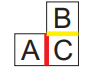
\includegraphics[width=0.1\textwidth]{img/sistemi_complessi/tileset.png}
            \end{figure}
            \begin{figure}
                \centering
                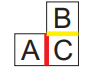
\includegraphics[width=0.1\textwidth]{img/sistemi_complessi/tileset.png}
            \end{figure}
        \end{itemize}
        Dimsotriamo le singole implicazioni:
        \begin{itemize}
            \item $\implies$: Se $T$ ammette tiling valido allora $q$ non compare 
            mai perché esiste sempre esattamente un $C$, quindi significa che $CA$
            non è nilpotente
            \item $\impliedby$: Ci si basa sul principio di compattezza del Tiling 
            negato. $T$ non ammette tiling valido allora tutti i quadrati di dimensione 
            $n\times n$ non sono validi per qualche $n$.
            
            Per ipotesi sappiamo che $T$ non è valido, questo significa che 
            per il principio di compattezza, una qualsiasi configurazione contiene 
            almento un $q$, quindi facendo evolvere l'automa otterremo prima o poi 
            la configurazione quiesciente.
        \end{itemize}    
    \end{proof}
\end{teorema}

Tutto quello che abbiamo detto vale anche per $NE, SW, SE$. Un tile set 
è $4$-way deterministic se è deterministico in ogni direzione.

\begin{nota}
    Possiamo costruire tileset aperiodico.
\end{nota}

\begin{teorema}
    Il tiling problem è indecidibile in tutte e $4$ direzioni.
\end{teorema}

\subsection{Snakes}

\begin{definizione} [\textbf{Snake} (directed tiles)]
    \textbf{Snake} è un tileset con l'aggiunta di frecce verso le 4 direzioni (N,W,E,S).
\end{definizione}

Dato un generico tiling di \textbf{Snake} (valido o no), a partire da una qualsiasi posizione
Dato un generico tiling di \textbf{Snake} (valido o no), a partire da una qualsiasi posizione
si possono generare dei cammini infiniti dati dalle freccie, questi possono 
essere:
\begin{itemize}
    \item infiniti senza loop
    \item infiniti con loop
\end{itemize} 

Sui cammini possono accadere le seguenti cose:
Sui cammini possono accadere le seguenti cose:
\begin{enumerate}
    \item ci può essere un tiling error tra due tiles entrambe sul percorso
    \begin{figure}[!h]
        \centering
        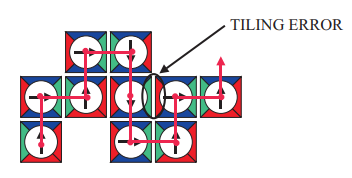
\includegraphics[width=0.5\textwidth]{img/sistemi_complessi/snake1.png}
    \end{figure}
    \begin{figure}[!h]
        \centering
        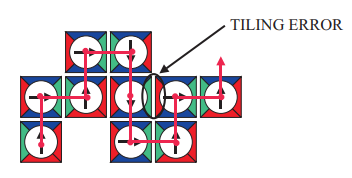
\includegraphics[width=0.5\textwidth]{img/sistemi_complessi/snake1.png}
    \end{figure}
    \item il percorso è un \textbf{plane-filling path}, ovvero $\forall n\in \mathbb{N}^+$
    esistono $n\times n$ quadrati incui tutte le loro posizioni vengono visitate 
    dal cammino.
    \begin{figure}[!h]
        \centering
        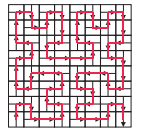
\includegraphics[width=0.2\textwidth]{img/sistemi_complessi/snake2.png}
    \end{figure}
    \begin{figure}[!h]
        \centering
        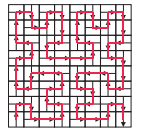
\includegraphics[width=0.2\textwidth]{img/sistemi_complessi/snake2.png}
    \end{figure}
\end{enumerate}



\begin{nota}
    Un percorso che forza gli \textbf{Snake} ad ammettere tiling valido è il \textbf{
        plane-filling Hillbert curve} (quello dell'immagine)
        plane-filling Hillbert curve} (quello dell'immagine)
\end{nota}

\begin{esempio}
    Un esempio di applicazione degli Snakes corrisponde ad un CA inietivo sulle configurazioni periodiche
    Un esempio di applicazione degli Snakes corrisponde ad un CA inietivo sulle configurazioni periodiche
    ma non iniettivo su tutte le configurazioni.
\end{esempio}

Sia $G_p$ la restrizione della regola globale $G$ di un CA 1D alle configurazioni 
periodiche allora 
si sa che
$$G \text{ iniettiva} \iff G_p \text{ iniettiva}$$
$$G \text{ suriettiva} \iff G_p \text{ suriettiva}$$

Nel caso bidimensionale si può solo 
$$G \text{ iniettiva} \implies G_p \text{ iniettiva}$$
$$G \text{ suriettiva} \impliedby G_p \text{ suriettiva}$$

Infatti gli Snake permettono di dimostrare che 
$$G \text{ iniettiva} \not\impliedby G_p \text{ iniettiva}$$

Gli Snake sono utili anche per provare l'indecidibilità che CA 2D sia reversibile.
La dimostrazione si basa sulla riduzione del tiling problem all'utilizzo degli 
Snake.

\begin{teorema}
    Il problema di determinare se CA 2D è reversibile (e quindi anche iniettivo)
    è indecidibile.
    \begin{proof}
        Dato un qualsiasi $T$ tileset, costruiamo un CA 2D (Snake XOR) nel seguente modo:
        \begin{itemize}
            \item alfabeto $S = T\times Snakes\times \{0,1\}$. Ogni cella è composta 
            da un tile di $T$, uno Snake tile e un bit, dove solo $T$ può variare e 
            $T$ e lo Snake hanno gli stessi colori.
            \item regola locale:
            \begin{itemize}
                \item tile error: se c'è un tile error la cella rimane invariata
                \item tile valido: la cella è attiva quindi il bit verrà aggiornato 
                calcolando lo XOR tra se stesso e il bit della cella puntata dalla 
                freccia dello Snake.
            \end{itemize}
        \end{itemize}

        Possiamo riportare il problema all'automa CA è reversibile sse il tile 
        set $T$ non ammette tile valido. 

        Dimostriamo le implicazioni:
        \begin{itemize}
            \item $\implies$: dimostriamo che $T$ ammette tile valido allora 
            CA non è reversibile.
            CA non è reversibile.

            Se $T$ ammette tile valido costruiamo $2$ configurazioni $c', c''$
            tali che $G(c') = G(c'')$. Lo Snake e $T$ hanno lo stesso tiling valido
            e $c'\ne c''$, per esempio $c'$ è composto da soli $0$ mentre $c''$ 
            è composto da soli $1$.

            Per entrambe le configurazioni le celle sono attive, perché 
            hanno lo stesso tiling corretto, quindi significa che si devono aggiornare.
            $G(c') = c'$ perché ha soli $0$, mentre $G(c'') = c'$ perché è composta 
            da soli $1$ che in XOR tra di loro ritornano sempre $0$. Quindi CA non 
            è iniettivo e di conseguenza non è reversibile.
            \item $\impliedby$: Dimostriamo che da CA non sia iniettivo si riesce 
            a dimostrare che ammette tiling valido.
                        
            supponiamo che CA non sia iniettivo, Sia $c$ e $d$
            due diffenti configurazioni con la stessa immagine. Questi 
            avranno $T$ e Snake identici e validi, quindi ahnno bit $0$ e $1$ differenti
            alla posizione $p_1\in \mathbb{Z}$.

            Dal momento che $c$ e $d$ hanno lo stesso successore:
            \begin{itemize}
                \item le celle in posizione $p_1$ devono essere attive perché
                Snakes e $T$ sono validi alla posizione $p_1$
                \item i bit nella posizione successiva $p_2$ puntata dallo Snake
                sono differenti in $c$ e $d$.
            \end{itemize}
            Possiamo continuare ricorsivamente con le stesse motivazioni.
            Avremo quindi una successione di $p_1,p_2,p_3\dots$ che seguono le 
            frecce. Non c'è nessun tiling error per tutto il percorso, quindi 
            è un \textbf{plane-filling path} di tiles validi quindi $T$ deve 
            ammettere tiling valido su tutto il piano
        \end{itemize}
    \end{proof}
\end{teorema}

Il tile è usato per principalmente per studiare problemi di autoassemblaggio di 
cellule (modello Winfree). In sostanza si aggiunge un tile alla volta al piano in modo che rimanga 
valido. Il piano piano continua a crescere irregolarmente fino a quando non possiamo 
più aggiungere tile, questo corrisponde all'autoassemblaggio biologico.

La regola di match in questo problema può essere di due tipi:
\begin{itemize}
    \item \textbf{strong matching rules}: ogni nuovo tile deve metchare con i colori 
    dei tile di tutti i vicini assemblati precedentemente
    \item \textbf{weak matching rules}: ogni nuovo tile deve metchare con i colori 
    dei tile di almeno un solo vicino assemblato precedentemente
\end{itemize}

\begin{definizione} [\textbf{Terminal assembly}]
    Un pattern è \textbf{terminal assembly} se non ha più tile che si possono aggiungere
\end{definizione}
\begin{definizione} [\textbf{Unbounded assembly}]
    Un tile set ammette un \textbf{unbounded assembly} se è un infinita sequenza 
    di tile aggiunti senza poter arrivare ad un terminal assembly possibile
\end{definizione}

\begin{teorema}
    Il problema di riconoscere se un tile ammette unbounded assembly è un problema decidibile.

    Questo problema coincide col cercare se esiste uno Snake che lo rappresenta.
\end{teorema}

Posiamo simulare una macchina di turing con un tiles set e il problema del tiling.
Definiamo un tile set composto da:
\begin{itemize}
    \item action tile
    \item merging tile 
\end{itemize}
Si rappresenta l'esecuzione della macchina mediante il nastro, ad ogni cella viene 
associata una piastrella. Ad ogni scatto della funzione utilizzeremo 
una piastrella action per la cella dalla quale abbiamo letto il carattere e metteremo
nella cella dove si sposterà la testina, una piastrella di merging. In questo modo 
una MT non si arresta per ogni input sse posso costruire un tile set valido.

\begin{nota}
    Le piastrelle non avranno i colori ma delle frecce entranti, uscenti o nessuna 
    freccia. Le frecce entranti rappresentano $qa$ lo stato attuale $q$ e il carattere 
    letto $a$. Le frecce uscenti $a'$ o $q'$ rappresentano rispettivamente il nuovo 
    carattere da scrivere e il nuovo stato.
\end{nota}

\begin{figure}[!h]
    \centering
    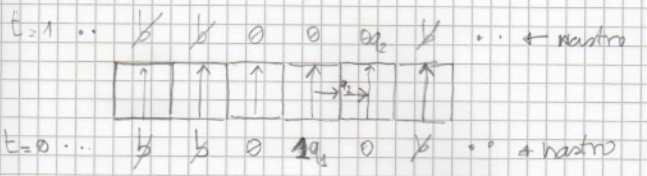
\includegraphics[width=0.5\textwidth]{img/sistemi_complessi/simulazione_mt_tile.png}
\end{figure}
\begin{figure}[!h]
    \centering
    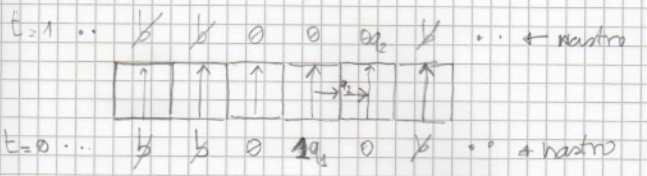
\includegraphics[width=0.5\textwidth]{img/sistemi_complessi/simulazione_mt_tile.png}
\end{figure}
\section{Subshift}

Modelli che permettono di codificare sequenze bi-infinite di caratteri escludendo 
delle parole finite (codifica con parole proibite). Usati per modellare il salvataggio
dei dati su disco fisso.

\begin{definizione} [\textbf{Sottostringa di una stringa bi-infinita}]
    Sia  $x\in A^\mathbb{Z}$ e una parola $w\in A^+$. Diremo che $w$ è sottostringa (finita) 
    di $x$ sse $\exists i,j\in \mathbb{Z}$ con $i\le j$ tale che $w=x_{[i,j]}$
\end{definizione}

\begin{definizione} [\textbf{Subshift}]
    Sia $X\subseteq A^\mathbb{Z}$ è un subshift sse $\exists \mathcal{F}\subseteq A^\ast$
    tale che $X= X_\mathcal{F}$
\end{definizione}

$X$ è generato da $\mathcal{F}$ e sarà composto da parole che non hanno come 
sottostringhe parole di $\mathcal{F}$. Spesso saremo interessati a cercare 
di rappresentare finitamente $X_\mathcal{F}$.

\begin{esempio}
    $X =  A^\mathbb{Z}$ è un subshift perché $\mathcal{F} = \emptyset$.
\end{esempio}

Sia $X\subseteq A^\mathbb{Z}$, non per forza un subshift
\begin{definizione} [\textbf{linguaggio di $X$}]
    Il \textbf{linguaggio di} $X$ è
    $$\mathcal{B}(X) = \bigcup_{n\in \mathbb{N}} \mathcal{B}_n(X)= \{w\in A^\ast| \exists x\in X, w\prec x\}$$
    Dove $\mathcal{B}_n(X) = \{w\in A^n| \exists x\in X, w\prec x\}$
\end{definizione}

\begin{definizione} [\textbf{Linguaggio fattoriale}]
    Il linguaggio $\mathcal{L}\subseteq A^\ast$ è \textbf{fattoriale} se $\forall
    u\in \mathcal{L}$, $w\prec u\implies w\in \mathcal{L}$

\end{definizione}


\begin{definizione} [\textbf{Linguaggio espandibile}]
    Il linguaggio $\mathcal{L}\subseteq A^\ast$ è \textbf{espandibile} se $\forall
    u\in \mathcal{L}$, $\exists v,w\in \mathcal{L}$ tale che $vuw\in \mathcal{L}$.
\end{definizione}

\begin{teorema}
    Sia $X\subseteq A^\mathbb{Z}$, $X$ è un \textbf{subshift} sse $\mathcal{B}(X)$ è 
    \textbf{fattoriale} e \textbf{espandibile}
\end{teorema}

\subsection{Subshift di tipo finito}
\begin{definizione} [\textbf{Subshift di tipo finito (SFT)}]
    Sia $X$ un subshift, $X$ è SFT se $\exists \mathcal{F}\subseteq A^\ast$ con
    $|\mathcal{F}|<\infty$ tale che $X= X_\mathcal{F}$
\end{definizione}

\begin{esempio}[\textbf{Golden Mean Shift}]
    $X=X_\mathcal{F}$ con $\mathcal{F} = \{11\}$ e $|\mathcal{F}|<\infty$, $X$ è
    SFT.
\end{esempio}

Per definire un subshift come $SFT$ allora basta che esista un insieme generatore
finito.
\begin{definizione}
    $X$ è un SFT di memoria $M$ se  $\mathcal{F}\subseteq A^{M+1}$ tale che $X=X_\mathcal{F}$.
\end{definizione}

\begin{esempio}[\textbf{Golden Mean Shift}]
    $X=X_\mathcal{F}$ con $\mathcal{F} = \{11\}\subseteq A^{1+1}$ è
    SFT di memoria $1$.
\end{esempio}

\begin{nota}
    se $X$ è memoria $M$ allora sarà anche a memoria $M+1,M+2,M+k,\dots$. Infatti 
    basta prendere la parola più lunga in $\mathcal{F}$ e completare le altre 
    con qualsiasi sinbolo di $A$.
\end{nota}

\begin{teorema}
    Sia $X$ un subshift di memoria $M$ e $x\in A^{\mathbb{Z}}$.
    $$x\in X\iff \forall i, x_{[i,i+M]}\in \mathcal{B}_{M+1}(X)$$
\end{teorema}
Si dice di memoria $M$ perché quando controllo se una parola appartiene al subshift
controllo a gruppi della sua lunghezza inserendo un simbolo in coda e rimuovendo un 
simbolo in testa.

\begin{definizione} [\textbf{Rappresentazione a blocchi}] 
    Sia $N\ge 1, N\in\mathbb{N}$. Una \textbf{Rappresentazione a blocchi} è $\beta_N:A^\mathbb{Z}\to (A^N)^\mathbb{Z}$
    tale che $\forall x\in A^\mathbb{Z}$:
    $$x=(\dots, x_{-1},x_0,x_1,x_2,x_3,x_4,\dots)$$
    $$\beta_N(x)=\left(\dots, \begin{array}{c}x_{-1}\\x_0\\\vdots\\x_{N-2}\end{array},\begin{array}{c}x_{0}\\x_1\\\vdots\\x_{N-1}\end{array},\begin{array}{c}x_{1}\\x_2\\\vdots\\x_{N}\end{array},\dots\right)$$
    quindi è come dire $\forall x\in A^\mathbb{Z}, \forall i \in \mathbb{Z}$:
    $$\beta_N(x)_i = \begin{array}{c}x_{i}\\x_{i+1}\\\vdots\\x_{i+N-1}\end{array}$$
\end{definizione}

\begin{definizione} [\textbf{Rappresentazione a blocchi di} $X$] 
    Sia $N\ge 1$. Una \textbf{Rappresentazione a blocchi di} $X$ è
     $$X^{[N]} =\beta_N (X)$$
    Sia $N\ge 1$. Una \textbf{Rappresentazione a blocchi di} $X$ è
     $$X^{[N]} =\beta_N (X)$$
\end{definizione}

\begin{teorema}
    $X^{[N]} $ è un subshift
\end{teorema}

\begin{esempio}
    Sia $\mathcal{F}=\{11\}$, $X = X_\mathcal{F}$ e sia $N=2$ allora 
    $$x=(\dots, 0,1,0,0,0,1,\dots)\in X$$
    $$\beta_2(x)=(\dots, 01,10,00,00,01,1\ast,\dots)\in X^{[2]}$$
    $$x=(\dots, 0,1,0,0,0,1,\dots)\in X$$
    $$\beta_2(x)=(\dots, 01,10,00,00,01,1\ast,\dots)\in X^{[2]}$$

    In generale $\beta_N(x)_i = x_{[i, i+N-1]}$
    In generale $\beta_N(x)_i = x_{[i, i+N-1]}$
\end{esempio}

\begin{definizione} [\textbf{Grafo di in SFT}]
    Il grafo di un SFT $X$ di memoria $M$ ($\exists \mathcal{F}\subseteq A^{M+1}, X= X_\mathcal{F}$) 
    è $G=(V,E)$ tale che:
    \begin{itemize}
        \item $V = \mathcal{B}_M(X)\subseteq A^M$
        \item $E = \{(u,v)\in V\times V | u = u_1\dots u_M, v= v_1\dots v_M,u_2\dots u_M = v_1\dots v_{M-1}\land uv_M= u_1v \not \in \mathcal{F}\}$ 
    \end{itemize}
\end{definizione}

La costruzione del grafo per un subshift $X$ di memoria $M$ si effettua nel seguente modo:
La costruzione del grafo per un subshift $X$ di memoria $M$ si effettua nel seguente modo:
\begin{itemize}
    \item Calcolo $\mathcal{B}_M(X)$ che sono i vertici
    \item Calcolo $\mathcal{B}_M(X)$ che sono i vertici
    \item disegno un arco tra due nodi solo se $u_1v=uv_M \not \in \mathcal{F}$
    \item controllo tutti i cammini biinfiniti e controllo che tutti gli archi 
    fanno parte dei cammini. Se non fanno parte allora si cancellano gli archi e i
    nodi isolati.
\end{itemize}
\begin{figure}[!h]
    \centering
    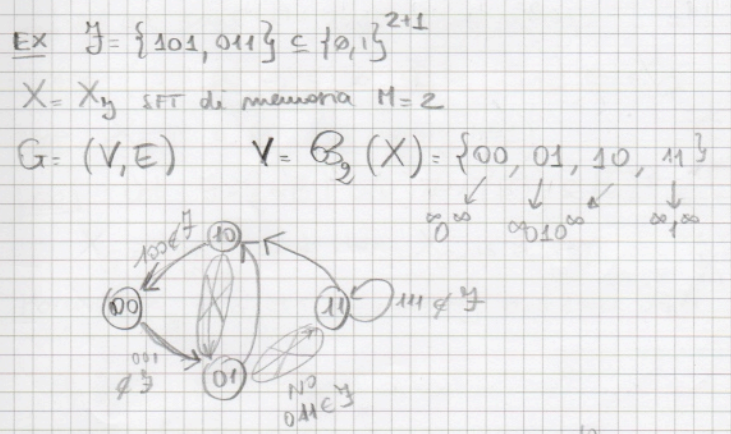
\includegraphics[width=0.4\textwidth]{img/sistemi_complessi/subshift.png}
\end{figure}

\begin{figure}[!h]
    \centering
    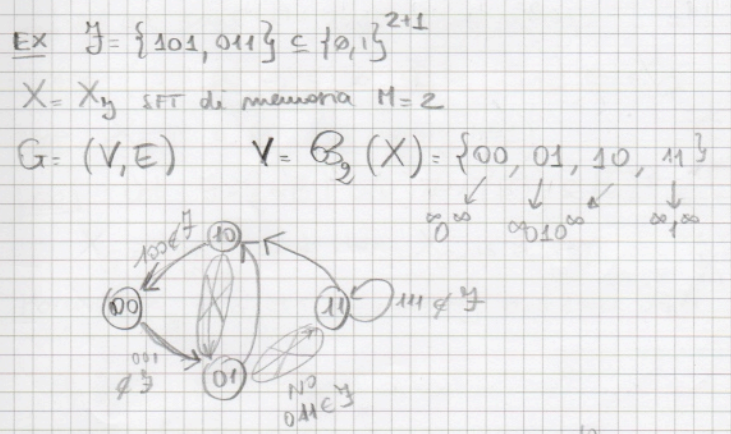
\includegraphics[width=0.4\textwidth]{img/sistemi_complessi/subshift.png}
\end{figure}


Il grafo è un sottografo del De Bruijn.

Dato un generico grafo $G=(V,E)$ possiamo ottenere un subshift $X_G$ che è SFT.
$$X_G=\{x\in E^\mathbb{Z}|\forall i\in\mathbb{Z}, t(x_i) = i(x_{i+1}) \}\equiv X^{[M+1]}$$
dove:
\begin{itemize}
    \item $t(\alpha)$ è il vertice terminale dell'arco $\alpha$
    \item $i(\alpha)$ è il vertice iniziale dell'arco $\alpha$
\end{itemize}

In sostanza $E^\mathbb{Z}$ sono tutti i cammini biinfiniti sugli archi composti dagli archi
stessi, non dalle label.

$x \in X_G$ è un cammino sugli archi di $G$ composto dal nome dei singoli archi attraversati ($A= E$).
Per definizione $x\in \beta_{M + 1}(y), \forall y\in X$.

\begin{teorema}
    $X_G$ è un SFT di memoria $M=1$.
    \begin{proof}
        Sia $\mathcal{F}= \{\alpha\beta|t(\alpha) \ne i(\beta)\}\subseteq E^2$ allora 
        si ha che $X_G= X_\mathcal{F}$ e allora $X_G$ è un SFT, inoltre è di memoria 
        $M=1$  perché $\mathcal{F}\subseteq A^{M+1=1+1}$.
        $M=1$  perché $\mathcal{F}\subseteq A^{M+1=1+1}$.
    \end{proof}
\end{teorema}
In generale ho $X$ di memoria $M$, costruisco $G$ e poi ottengo $X_G = X^{[M+1]}$ che contiene gli 
In generale ho $X$ di memoria $M$, costruisco $G$ e poi ottengo $X_G = X^{[M+1]}$ che contiene gli 
archi. Al contrario se prendo tutti i cammini sui vertici allora ottengo lo stesso
subshift ma nella rappresentazione a blocchi $X^{[M]}$

Ora consideriamo il grafo $\mathcal{G}=(V,E,l)$ con $l:E\to A$ un grafo etichettato 
tale che $G=(V,E)$.
\begin{definizione}
    $l_\infty:E^\mathbb{Z}\to A^\mathbb{Z}$ tale che 
    $$\forall x\in E^\mathbb{Z}, \forall i \in \mathbb{Z}, l_\infty(x)_i = l(x_i)$$
\end{definizione}
\begin{nota}
    $l_\infty$ è l'estensione alle stringhe biinfinite di $l$.
\end{nota}

\begin{definizione}
    $X_\mathcal{G}= \{y\in A^\mathbb{Z}|\exists x\in E^\mathbb{Z} : \forall i\in \mathbb{Z}, t(x_i) = i(x_{i+1})\land y_i=l(x_i)\}=l_\infty(X_G)$.
    $X_\mathcal{G}= \{y\in A^\mathbb{Z}|\exists x\in E^\mathbb{Z} : \forall i\in \mathbb{Z}, t(x_i) = i(x_{i+1})\land y_i=l(x_i)\}=l_\infty(X_G)$.
    In sostanza sono i cammini di $X_G$ ma sostituendo gli archi con le etichette.
\end{definizione}

\begin{osservazione}
    $y\in X_\mathcal{G}$ sse cammino biinfinito sulle etichette degli archi di $\mathcal{G}$
\end{osservazione}
\begin{nota}
    $X_\mathcal{G}$ è un subshift
    \begin{proof}
        $X_\mathcal{G} = X_\mathcal{F}$ con $\mathcal{F}=\mathcal{B}(X_\mathcal{G})^C$
        dove il complemento è rispetto ad $A^\ast$
    \end{proof}
\end{nota}


\begin{definizione}
    $X$ è \textbf{Sofico} sse $\exists \mathcal{G}$ tale che $X= X_\mathcal{G}$
\end{definizione}

I sofici hanno una rappresentazione finita perché $X_\mathcal{G}$ è una rappresentazione 
finita. 

\begin{definizione}
    $\mathcal{G}$ si dice right resolving se $\mathcal{G}$ è il
    grafo di un automa a stati finiti deterministico.     
\end{definizione}

Se il grafo non è deterministico possono trasformarlo. Quindi SFT $\subseteq$ sofici.

Da un $X$ possiamo costruire un $G$ allora possiamo ottenere $\mathcal{G}$ usando solo
come etichette la stringa associata al vertice di partenza. Se guardiamo i camminmi biinfiniti sulle
etichette allora ottengo il subshift che è la sua rappresentazione a blocchi $1$ (vedi \ref{fig:subshift}).  

\begin{figure}[!h]
    \centering
    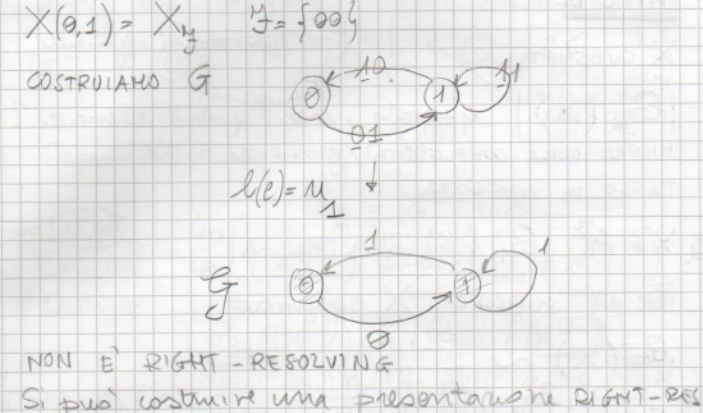
\includegraphics[width=0.5\textwidth]{img/sistemi_complessi/subshift_e_grafi.png}
    \caption{Esempio di otteniumento di un grafo di un subshift}
    \label{fig:subshift}
\end{figure}
come etichette la stringa associata al vertice di partenza. Se guardiamo i camminmi biinfiniti sulle
etichette allora ottengo il subshift che è la sua rappresentazione a blocchi $1$ (vedi \ref{fig:subshift}).  

\begin{figure}[!h]
    \centering
    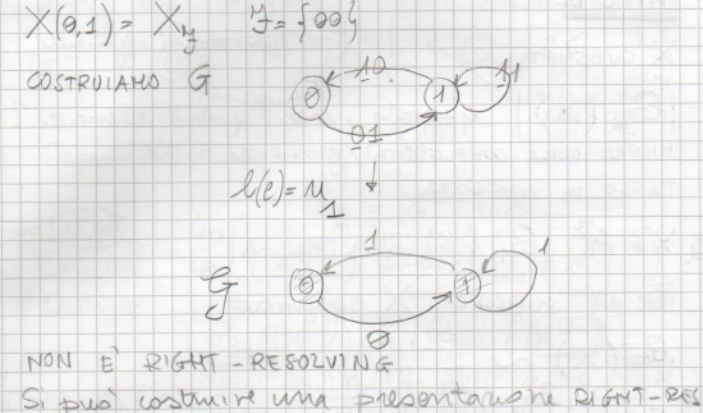
\includegraphics[width=0.5\textwidth]{img/sistemi_complessi/subshift_e_grafi.png}
    \caption{Esempio di otteniumento di un grafo di un subshift}
    \label{fig:subshift}
\end{figure}

\subsection{Entropia}
Sia $X$ un subshift, come possiamo sapere quanto cresce $|\mathcal{B}_n(X)|$, tasso
di crescita si può misurare, infatti se $X=A^\mathbb{Z}$ allora $|\mathcal{B}_n(X)|=|A^n|= 2^{\log_2|A|n}$.
Se $A$ è un alfabeto binario. La componente che ci interessa è $\log_2 |A|$ perché
è quello che varia tra subshift, quindi per un subshift $X$ qualunque su alfabeto binario
allora posso dire che $|\mathcal{B}_n(X)| \sim 2^{cn}$ quindi $c\sim \frac{\log_2|\mathcal{B}_n(X)|}{n}$.

\begin{definizione}
    L'\textbf{entropia} di un subshift $X$ è 
    $$h(X) = \lim_{n\to \infty}\frac{\log_2|\mathcal{B}_n(X)|}{n}$$
\end{definizione}
Questo limite esiste (sarebbe da dimostrare).
Questo limite esiste (sarebbe da dimostrare).

\begin{nota}
    $h(X)\le \log_2|A|$ infatti
    $|\mathcal{B}_n(X)| \le |A|^n\iff \log_2 |\mathcal{B}_n(X)| \le \log_2 |A|^n \iff
    \frac{\log_2|\mathcal{B}_n(X)|}{n}\le \log_2|A|\iff h(X)\le \log_2|A|$.
    $|\mathcal{B}_n(X)| \le |A|^n\iff \log_2 |\mathcal{B}_n(X)| \le \log_2 |A|^n \iff
    \frac{\log_2|\mathcal{B}_n(X)|}{n}\le \log_2|A|\iff h(X)\le \log_2|A|$.
    Inoltre $h(A^\mathbb{Z}) = \lim_{n\to \infty}\frac{\log_2|A^n|}{n} =  \lim_{n\to \infty}\log_2|A| = \log_2|A|$.
    Quindi l'entropia massima è $\log_2|A|$.
\end{nota}

\begin{esempio}
    Sia $X=X_\mathcal{F}$ con $\mathcal{F} = \{11\}$ con $M=1$, vogliamo calcolare 
    Sia $X=X_\mathcal{F}$ con $\mathcal{F} = \{11\}$ con $M=1$, vogliamo calcolare 
    $h(X)$.

    Costruiamo $G$, otteniamo la matrice delle adiacenze $A=\left[\begin{array}{cc}
        1&1\\
        1&0
    \end{array}\right]$.

    Sappiamo che $X_G = X^{[2]}$ sono i cammini sugli archi, mentre il subshift ottenuto dai cammini
    sui vertici è $\hat{X}_G = X^{[1]} =X$.


    Sappiamo che $X_G = X^{[2]}$ sono i cammini sugli archi, mentre il subshift ottenuto dai cammini
    sui vertici è $\hat{X}_G = X^{[1]} =X$.

    Inoltre $\mathcal{B}_n(X^{[M]})$ è in corrispondenza biunivoca con $\mathcal{B}_{n-1}(X^{[M+1]})$,
    quindi possiamo dire che $|\mathcal{B}_n(X^{[1]})| = |\mathcal{B}_{n-1}(X^{[2]})|$ 
    ovvero $|\mathcal{B}_n(X)| = |\mathcal{B}_{n-1}(X_G)|$. 
    Allora $h(X)=\lim_{n\to \infty}\frac{\log_2|\mathcal{B}_n(X)|}{n} = \lim_{n\to \infty}\frac{\log_2|\mathcal{B}_{n-1}(X_G)|}{n}$.
    quindi possiamo dire che $|\mathcal{B}_n(X^{[1]})| = |\mathcal{B}_{n-1}(X^{[2]})|$ 
    ovvero $|\mathcal{B}_n(X)| = |\mathcal{B}_{n-1}(X_G)|$. 
    Allora $h(X)=\lim_{n\to \infty}\frac{\log_2|\mathcal{B}_n(X)|}{n} = \lim_{n\to \infty}\frac{\log_2|\mathcal{B}_{n-1}(X_G)|}{n}$.
\end{esempio}
Ogni elemento di $\mathcal{B}_{m}(X_G)$ corrisponde ad una parola di lunghezza 
$m$ che si ottiene come cammino di lunghezza $m$ sugli archi, quindi 
$m$ che si ottiene come cammino di lunghezza $m$ sugli archi, quindi 
$|\mathcal{B}_{m}(X_G)|$ è il numero di cammini di lunghezza $m$ tra coppie qualunque
di vertici di $G$.
$$|\mathcal{B}_{m}(X_G)| = \sum_{i\in V}\sum_{j\in V} a_{ij}^{(m)}$$
Dove $a_{ij}^{(m)}$ è un elemento di $A^m$.

Risulta quindi utile trovare un modo per calcolare velocemente $A^m$, questo può
essere fatto con la diagonalizzazione, infatti se tendiamo di diagonalizzare $A$ ($A=PDP^{-1}$),
possiamo calcolare $A^m=PD^{m}P^{-1}$ dove $D$ è la matrice diagonale degli autovalori
e $P$ è la matrice degli autovettori associati agli autovalori. Essendo diagonale 
$D^m$ coincide con l'elevazione a potenza degli autovalori.

Per diagonalizzare $A$ dobbbiamo:
\begin{itemize}
    \item calcolare gli autovalori ottenendo il polinomio caratteristico $det(A-\lambda Id) =0$.
    \item calcolo gli autovettori
    \item risolvo il prodotto tra matrici
\end{itemize}

In questo modo possiamo poi calcolare l'entropia del subshift
$$h(X)=\lim_{n\to \infty}\frac{\log_2|\mathcal{B}_n(X)|}{n} = \lim_{n\to \infty}\frac{\log_2|\mathcal{B}_{n-1}(X_G)|}{n} = \lim_{n\to \infty}\frac{\log_2\sum_{i\in V}\sum_{j\in V} a_{ij}^{(n-1)}}{n} $$

In questo modo possiamo poi calcolare l'entropia del subshift
$$h(X)=\lim_{n\to \infty}\frac{\log_2|\mathcal{B}_n(X)|}{n} = \lim_{n\to \infty}\frac{\log_2|\mathcal{B}_{n-1}(X_G)|}{n} = \lim_{n\to \infty}\frac{\log_2\sum_{i\in V}\sum_{j\in V} a_{ij}^{(n-1)}}{n} $$

\begin{teorema}
    Se $\mathcal{G}= (G,l)$ è right resolving allora $h(X_\mathcal{G}) = h(X_G)$
    Se $\mathcal{G}= (G,l)$ è right resolving allora $h(X_\mathcal{G}) = h(X_G)$
\end{teorema}

\begin{definizione}
    Sia $A\ge 0$ (ogni entry $\ge 0$) è \textbf{irriducibile} sse $\forall i,j,\exists n$ 
    Sia $A\ge 0$ (ogni entry $\ge 0$) è \textbf{irriducibile} sse $\forall i,j,\exists n$ 
    tale che $(A^n)_{ij}>0$.
\end{definizione}
\begin{teorema}
    Sia $G$ un grafo e $A$ la sua matrice di adiacenza allora $G$ è \textbf{fortemente 
    connesso} $\iff$ $A$ è irriducibile.
    Sia $G$ un grafo e $A$ la sua matrice di adiacenza allora $G$ è \textbf{fortemente 
    connesso} $\iff$ $A$ è irriducibile.
\end{teorema}
\begin{teorema} [\textbf{Perron Frobenius}]
    Sia $A\ne 0$ matrice irriducibile allora:
\begin{teorema} [\textbf{Perron Frobenius}]
    Sia $A\ne 0$ matrice irriducibile allora:
    \begin{itemize}
        \item $\exists v_A>0$ autovettore con corrispondente autovalore $\lambda_A>0$
        semplice (molteplicità algebrica $1$, è una sola radice)
        \item $\forall \mu $ autovalore di $A$ allora $|\mu| \le\lambda_A$
        \item $\forall v'>0$ autovettore di $A$, $v'$ è multiplo positivo di $v_A$
    \end{itemize}
    Quindi $\lambda_A$ è l'autovalore $>0$ di modulo massimo tra tutti gli autovalori 
    di $A$
\end{teorema}
\begin{teorema}
    $G$ grafo e $A$ sua matrice di adiacenza allora:
    \begin{itemize}
        \item $G$ è fortemente connesso $\implies h(X_G) = \log\lambda_A$
        \item $X$ SFT con grafo associato $G$ fortemente connesso $\implies h(X) = \log\lambda_A$
        \item $X$ sofico tale che $X=X_\mathcal{G}$ con $\mathcal{G} = (G,l)$ right 
        resolving e $G$ fortemente connesso $\implies h(X)=\log \lambda_A$

        resolving e $G$ fortemente connesso $\implies h(X)=\log \lambda_A$

    \end{itemize}
\end{teorema}
Per calcolare l'entropia di un subshift che è:
\begin{itemize}
    \item SFT con grafo $G$ fortemente connesso
    \item un sofico $X$ con $X=X_\mathcal{G}$ tale che è right resolving e $G$ fortemente
    connesso
\end{itemize}
è sufficiente calcolare l'autovalore di modulo massimo $\lambda_A>0$ allora $h(X)=\log_2\lambda_A$

\section{Codici}
\begin{definizione} [\textbf{Road-coloring}]
    Il \textbf{road-coloring} di un grafo $G=(V,E)$ è $l:E\to A$ tale che $\forall
    i\in V$ $|\{(i,j)\in E|j\in V\}| = |A|$ ovvero si ha una corrispondenza biunivoca tra $\{(i,j)\in E|j\in V\}$ e $A$
    (per ogni nodo abbiamo un numero di edge uscenti pari a $|A|$)
    (per ogni nodo abbiamo un numero di edge uscenti pari a $|A|$)
\end{definizione}
\begin{nota}
    $\forall w \in A^\ast$ e $\forall i\in V$ c'è un unico cammino. 
\end{nota}
\begin{definizione} [\textbf{Right-closing}]
    $G = (V,E,l)$ con $l:E\to A$ è \textbf{right-closing} con ritardo $D$ se $\forall \pi,\pi'$
\begin{definizione} [\textbf{Right-closing}]
    $G = (V,E,l)$ con $l:E\to A$ è \textbf{right-closing} con ritardo $D$ se $\forall \pi,\pi'$
    $\pi = e_1\dots e_De_{D+1},\pi' = e_1'\dots e_D'e_{D+1}'$ che partono dallo 
    stesso vertice $l(\pi)=l(\pi')\implies e_1=e_1'$
\end{definizione}
significa che dati due cammini sugli archi, l'etichettatura è right-closing se gli archi hanno la 
stessa mappatura allora hanno il primo arco in comune e poi hanno un fork con $D$ 
significa che dati due cammini sugli archi, l'etichettatura è right-closing se gli archi hanno la 
stessa mappatura allora hanno il primo arco in comune e poi hanno un fork con $D$ 
archi separati ma sempre con la stessa mappatura.
\begin{nota}
    Se $G = (V,E,l)$  è un grafo con $l:E\to A$ right-closing allora $\forall I\in V,
    Se $G = (V,E,l)$  è un grafo con $l:E\to A$ right-closing allora $\forall I\in V,
    \forall e,e'\in E^\mathbb{N}$ commini mono-infiniti uscenti da $I$, $l_\infty(e) = l_\infty(e') \implies e=e'$
\end{nota}
Se noi restringiamo $l_\infty$ al vertice $I\in V$ (funzione ristretta ai soli 
cammini mono-infiniti che partono da $I$) allora la funzione è iniettiva.

\begin{definizione}
    Un \textbf{codice a stati finiti} è una tripla $(G,I,O)$ tale che:
    \begin{itemize}
        \item $G$ è un grafo
        \item $I$ è il road-coloring di $G$ (input labeling)
        \item $O$ è il right-closing di $G$ (output labeling)
        \item $I$ è il road-coloring di $G$ (input labeling)
        \item $O$ è il right-closing di $G$ (output labeling)
    \end{itemize}
\end{definizione}

\begin{definizione}
    Un \textbf{codice a stati finiti} è anche una coppia $(X,n)$ con $X$ subshift in cui:
    \begin{itemize}
        \item $G$ associato a $X$ ha outdegree costante pari a $n$ 
        \item $X$ contiene $O_\infty(X_G)=\{y | \exists x\in X_G:\forall i,y_i=O(x_i)\}$ ($O_\infty(X_G)$ è sofico)
        \item $X$ contiene $O_\infty(X_G)=\{y | \exists x\in X_G:\forall i,y_i=O(x_i)\}$ ($O_\infty(X_G)$ è sofico)
    \end{itemize}
\end{definizione}
Si può usare un codice a stati finiti $(X,n)$ per trasformare sequenze di $A^\mathbb{N}$
Si può usare un codice a stati finiti $(X,n)$ per trasformare sequenze di $A^\mathbb{N}$
con $|A|=n$ in sequenze di $X$.

\begin{esempio}
    \begin{figure}[!h]
    \begin{figure}[!h]
        \centering
        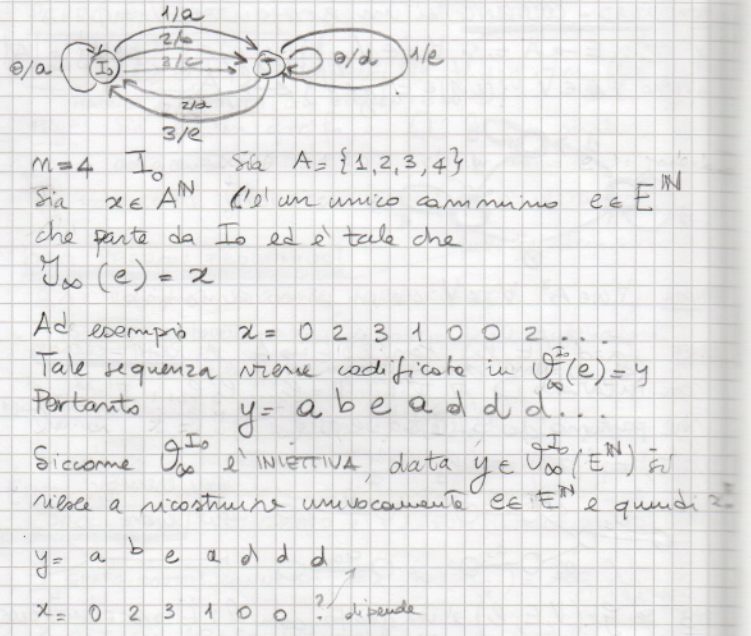
\includegraphics [width=0.5\textwidth]{img/sistemi_complessi/codici.png}
    \end{figure}
\end{esempio}

\begin{teorema}
    Sia $X$ un subshift sofico e $n\ge 1$. Esiste un codice a stati finiti 
    $$(X,|A|)\iff h(X)\ge \log_2 |A|$$
\end{teorema}
Il problema è che con alfabeti binari non si riuscirà mai ad avere $h(X) \ge \log_2 2$,
perché per definizione  si avrà sempre $h(X)< \log_2 2$. Per risolvere questo 
problema si può dividere l'input in blocchi di lunghezza $p$ e dividere l'output
in blocchi di lunghezza $q$, questa rappresentazione non è quella a blocchi perché
in questo caso i blocchi sono tutti disgiunti.

\begin{definizione} [\textbf{Power Shift}]
    Dato $N\ge 1$ allora 
    $$\gamma _N: A^{\mathbb{Z}} \to A^{N^{\mathbb{Z}}} $$
    o corrispondentemente $\gamma _N: A^{\mathbb{N}} \to A^{N^{\mathbb{N}}} $.

    $$\forall x \in A^{\mathbb{Z}}, \forall i \in \mathbb{Z} \gamma_N(x)_i = x_{[iN,iN+N -1]}$$
    o corrispondentemente $\forall x \in A^{\mathbb{N}}, \forall i \in \mathbb{N} \gamma_N(x)_i = x_{[iN,iN+N -1]}$
\end{definizione}
\begin{esempio}
    Supponiamo di avere $N=4$ allora
    $$x= \left(\dots, x_0,x_1,x_2,x_3,x_4,\dots\right)$$
    $$\gamma_4(x) = \left(\dots, \left(\begin{array}{c}
        x_0\\x_1\\x_2\\x_3
    \end{array}\right),\left(\begin{array}{c}
        x_4\\x_5\\x_6\\x_7\\
    \end{array}\right),\dots\right)$$
\end{esempio}
\begin{esempio}
    Supponiamo di avere $N=4$ allora
    $$x= \left(\dots, x_0,x_1,x_2,x_3,x_4,\dots\right)$$
    $$\gamma_4(x) = \left(\dots, \left(\begin{array}{c}
        x_0\\x_1\\x_2\\x_3
    \end{array}\right),\left(\begin{array}{c}
        x_4\\x_5\\x_6\\x_7\\
    \end{array}\right),\dots\right)$$
\end{esempio}
\begin{nota}
    $\gamma_N$ è applicabile non cecessariamente agli elementi dell'intero $A^\mathbb{Z}$ ($A^\mathbb{N}$),
    ma anche ad elementi di un subshift.
\end{nota}

Quindi dato un subshift $X\subseteq A^{\mathbb{Z}}$ ($A^{\mathbb{N}}$), si può
considerare $\gamma_N(X)$ che si indica con $X^N$ è chiamato Power shift di $X$

\begin{teorema}
    Se $X\subseteq A^\mathbb{Z }$ ($A^\mathbb{N}$) è un subshift allora 
    $$X^N= \gamma_N(X)=\{\gamma_N(x)|x\in X\}\subseteq (A^N)^\mathbb{Z} ((A^N)^\mathbb{N})$$
    $X^N$ è un subshift. Inoltre $h(X^N)=N\cdot h(X)$
\end{teorema}

Quindi tornando al problema di codificare l'alfabeto binario, possiamo codificare 
blocchi $\{0,1\}^\mathbb{N}$ in sequenze di un subshift buono $X$, ma in questo 
caso avremo sequenze 
blocchi $\{0,1\}^\mathbb{N}$ in sequenze di un subshift buono $X$, ma in questo 
caso avremo sequenze 
$\gamma_p(\{0,1\}^\mathbb{Z})$ da codificare in sequenze di $\gamma_q(X=X^q)$
con $p,q$ da determinare.

Il problema è trovare quanto devono valre $p,q$ affinché esista un codifice a stati 
finiti $(\gamma_q(X),n)$ dove stavolta $n=2^p$ in quanto le sequenze da codificare 
appartengono a $\gamma_p(\{0,1\}^\mathbb{N}) = (\{0,1\}^p)^\mathbb{N}$, cioè 
che appartengono al full shift sull'alfabeto $\{0,1\}^p$ anziché al full Shift
sull'alfabeto $\{0,1\}$.

Pertanto $n=|\{0,1\}^p| = 2^p$. Affinche esista un codice a stati finiti 
$(\gamma_q(X), n =2^p )$ che codifichi sequenze da $(\{0,1\}^p)^\mathbb{N}$ in 
$X^q=\gamma_q(X)$ occorre che $h(X^q)\ge \log_2n$ ossia che $q\cdot h(X)\ge \log_2 (2^p)$
cioè che $h(X)\ge \frac{p}{q}$.

In definitiva basta segliere $p$ e $q$ in modo tale che valga 
$$h(X)\ge \frac{p}{q} $$


$$h(X)\ge \frac{p}{q} $$

